\chapter{Promoting Unselfish Routes}
\label{ChapterPreTrip}

Traffic congestion has been a perennial problem in many highly urbanized cities across the globe. As government stakeholders tackle this issue by implementing policies and building infrastructure, they are also becoming aware that there is a greater need to promote sustainable driving behaviors among its citizen drivers to fully achieve their goals\cite{Attard2016TheSystems,darnton2008gsr}. It would take long term transformations on the route choice behavior of everyday drivers.

Navigation applications have a great potential in helping cities manage traffic flow at the onset of a traffic congestion. Drivers who commute daily to and from their work, school or business can be distributed and guided to a number of alternative routes with the goal of preventing traffic jams. If the road network is already experiencing traffic congestion on some of its roads, drivers can be directed to less used roads. And crucial to this is the timely delivery of navigational information that will aid the driver in their decision making. 

There are a number of factors that affect individual route choice \cite{Ben-Elia2015ResponseReview,Chorus2006TravelReview}. Arguably, the most important factor is travel time\cite{Ben-Elia2015ResponseReview} and we see this information constantly highlighted whenever we search for driving directions in most modern applications. While this is especially true in urgent circumstances, we found in Chapter \ref{ChapterInteractNavi} that in most cases, road and route familiarity and their closeness to what drivers use regularly play a bigger role in the decision making process. For these reasons, it can be a challenge if we suggest unselfish routes to daily commuters. Unlike optimal routes that are recommended because they have the fastest travel time or shortest distance, unselfish routes are alternatives that are typically sub-optimal (slower or longer). So now the question is if it would be possible to convince drivers to choose a sub-optimal unselfish route over an optimal one at the beginning of a trip. In this chapter, I:
\begin{itemize}
    \item describe a GUI-based approach that uses different combinations of motivative and familiarity information to route recommendations;
    \item show how these types of information and their combinations give promise for autonomy support for an unselfish route choice;
    \item elaborate how their causality orientations and behavioral regulatory styles explain their individual route choice; 
    \item discuss how participants were more likely to choose an unselfish route when presented with simple and explicit descriptions of its possible outcomes; and
    \item discuss how more support for relatedness is needed for drivers with moderate impersonal and controlled orientation.
\end{itemize}

To end this chapter, I argue the need for a more personalized motivation. In coming up with personalized and theory-based information displays, designers must be cautious as to how they will be interpreted. This is besides making sure that the information are properly supporting a psychological need. I also suggest exploring other types of information to support the basic psychological needs and other ways of presenting them (e.g. how to display on map?).

% I describe the different SDT-based motivative information that were added to route choices before a trip. Because unselfish routes may be perceived as a novel, sub-optimal choice by drivers, I also describe the additional information about route familiarity. I explore the effects of combining these motivative and familiarity navigational information on their route choice through a within-subject online experiment with 28 participants. They were asked to choose between an optimal and an unselfish route for 28 times under different conditions. it was found that all combinations of motivative and familiarity information showed significant 

\section{Review of Behavior Change Techniques}
In the Antecedent-Behavior-Consequence (ABC) model of behavior, antecedents are stimuli or events that trigger a current or target behavior. Behavior theories characterize them as psychological factors like motivation, self-efficacy, attitudes and benefits and risk perceptions, which can be influenced by a number of techniques. In traditional behavioral psychology, interventions can be delivered through personal interactions or other types of media (social influence). On the other hand, technology-based interventions are delivered through HCI or computer-mediated communication. As I described in Chapter \ref{ChapterRL}, HCI researchers continue to develop technology-based interventions, most of them targeted towards health, well-being, sustainability and privacy behavior outcomes. In Chapter \ref{ChapterSDT}, I also discussed how it is being used to increase motivation for active and continuous use of and participation in civic technologies. 

An early review of behavior change technologies by Hekler et. al. revealed that even though HCI researchers draw on behavior theories to derive design decisions, translating them into single features or full-blown applications and technologies still remain trivial\cite{hekler2013mind}. They argue that there has to be better bridging efforts whenever we design new technologies. Cowan et. al. found health and fitness applications to lack engagement with theory when they performed content analysis of app descriptions\cite{cowan2013apps}. This is further echoed by Tyack and Mekler in their systematic review of HCI games research\cite{tyack2020self}. They found that SDT-based game designs were mostly focused on needs satisfaction and intrinsic motivation, and other important mini-theories, like the Causal Orientation Theory, were rarely engaged with. 

However, HCI researchers also innovate on behavior change interventions without strict reference to theory, as this can open opportunities to extend existing theories or introduce new ones. And in order to scope how far innovations on behavior change have gone and what directions the field can go next, there were several attempts to classify them in categories. In the work of Lister et. al., they identified 13 behavior change constructs after looking into different gamification strategies used to promote physical activities and healthy diets\cite{lister2014just}. Stawarz et. al. found 10 classes of behavior change techniques used by commercial applications for habit formation\cite{stawarz2014don}. With a focus on health, Edwards et. al. examined applications that use gamification methods to promote health outcomes, and found 16 types of behavior change techniques used\cite{edwards2016gamification}. Aside from developing techniques that trigger target behaviors, another critical aspect that leads to successful behavior change is consistency in user engagement. In the most recent work of Caraban et. al., they found 23 nudging techniques and grouped them to the following 6 categories: facilitate, confront, deceive, social influence, reinforce, and fear\cite{caraban201923}. 

\begin{figure}[t]
\centering
  
\includegraphics[scale=0.8]{figures/s3-navi-parts.png}
  \caption{The motivative and familiarity information added to the typical travel information for each route recommendation.}~\label{fig:s3-new-info}
\end{figure}

Although previous findings suggest that such technology-based interventions have resulted to some changes in behavior, most can only claim modest effectiveness. One possible reason is that the techniques we introduce might not be the most effective in changing the antecedents or psychological factors that promote a target behavior. Aside from the domain-specific classifications discussed above, this issue can be resolved with the development and use of taxonomies. As a first attempt, Abraham and Michie developed a taxonomy of 26 behavior change techniques that allowed other researchers to identify the different components of proposed interventions\cite{abraham2008taxonomy}. Since then, it has been widely adopted by many researchers, but conceptual problems and overlaps in definitions were later discovered. This was addressed by the CALO-RE taxonomy which now includes 40 clearly defined behavior change techniques\cite{michie2011refined}. Working with a larger team, Michie et. al. expanded the taxonomy further with 93 behavior change techniques that are hierarchically structured, which they named ``BCT Taxonomy v1''\cite{michie2013behavior}. Unlike previous versions of the taxonomy, this step change has international consensus, but they indicate that there will be more development and evaluation. Besides taxonomies, Oinas-Kukkonen et. al. also introduced 28 principles that are part of the Persuasive Systems Design Framework\cite{oinas2009persuasive}. In this dissertation, I used the CALO-RE\cite{michie2011refined} and BCT Taxonomy V1\cite{michie2013behavior} as main reference for the proposed techniques. For the pre-trip approach discussed in this chapter, the behavior change technique of information provision is used by adding two new sets of information to describe both routes and their possible outcomes when chosen and followed (Figure \ref{fig:s3-new-info}). The first is motivative while the other shows familiarity. 

\section{Motivative Information}
In order to promote the use of unselfish routes without any explicit messaging diversification and incentive structures, the addition of relevant navigational information must support the three basic psychological needs for autonomy, competence, and relatedness. Figure \ref{fig:s3-motivative} shows the three types of motivative information used in this approach: critical mass, valence framing, and simple positive framing. Each type of information is aligned with techniques 1, 2 \& 4 of the CALO-RE taxonomy\cite{michie2011refined} and the different information provision techniques under codes 5 (\textit{Natural Consequences}) and 6 (Comparison of Behaviour) of BCT Taxonomy V1\cite{michie2013behavior}. The following subsections will discuss the rationale behind each type of motivative information and the limitations and nuances in their design.

\begin{figure}[t]
\centering
  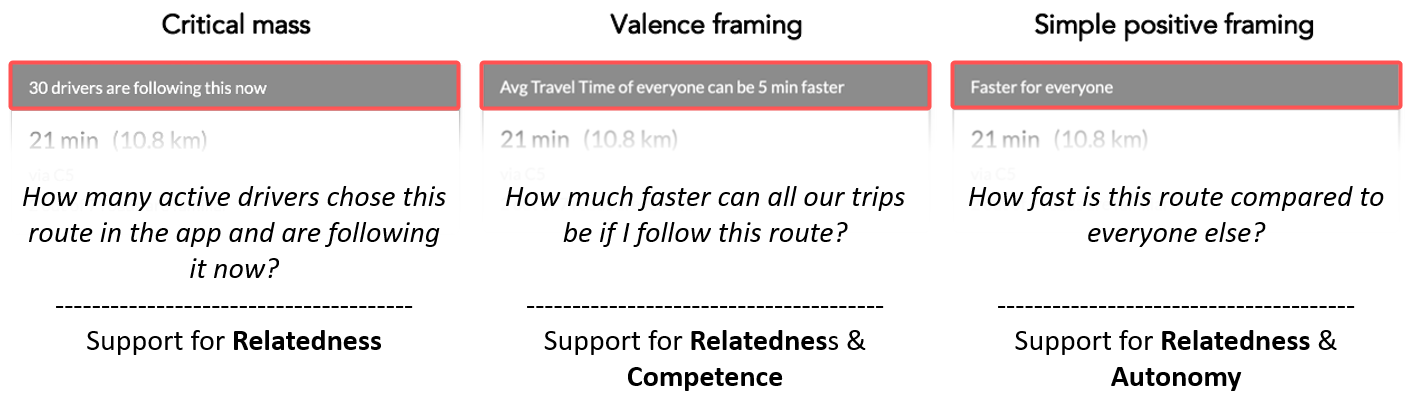
\includegraphics[scale=0.6]{figures/s3-motivative.png}
  \caption{The three types of motivative information used. At the bottom of each design are the basic psychological needs supported by the information provided.}~\label{fig:s3-motivative}
\end{figure}

% \begin{table}[h]
%     \caption{The types of motivative information.}
% 	\label{tab:motive-info}
% 	\centering
% 	\begin{tabular}{l l}
% 	    \hline\hline
% 		\textbf{Motivative Information} & \textbf{Template} \\
% 		\hline
% 		\textbf{Critical mass} & \textbf{Optimal} \\
% 		& 70 drivers are following this now. \\
% 		& \textbf{Unselfish} \\
% 		& 30 drivers are following this now. \\
%         \textbf{Valence framing} & \textbf{Optimal} \\
%         & Avg Travel Time of everyone can be 0 min faster \\
% 		& \textbf{Unselfish} \\
% 		& Avg Travel Time of everyone can be <N> min faster \\
%         \textbf{Simple positive framing} & \textbf{Optimal} \\
%         & Fastest for you \\
% 		& \textbf{Unselfish} \\
% 		& Faster for everyone \\
% 		\hline
% 	\end{tabular}
% \end{table}

\subsection{Critical Mass}
\begin{figure}[h]
\centering
  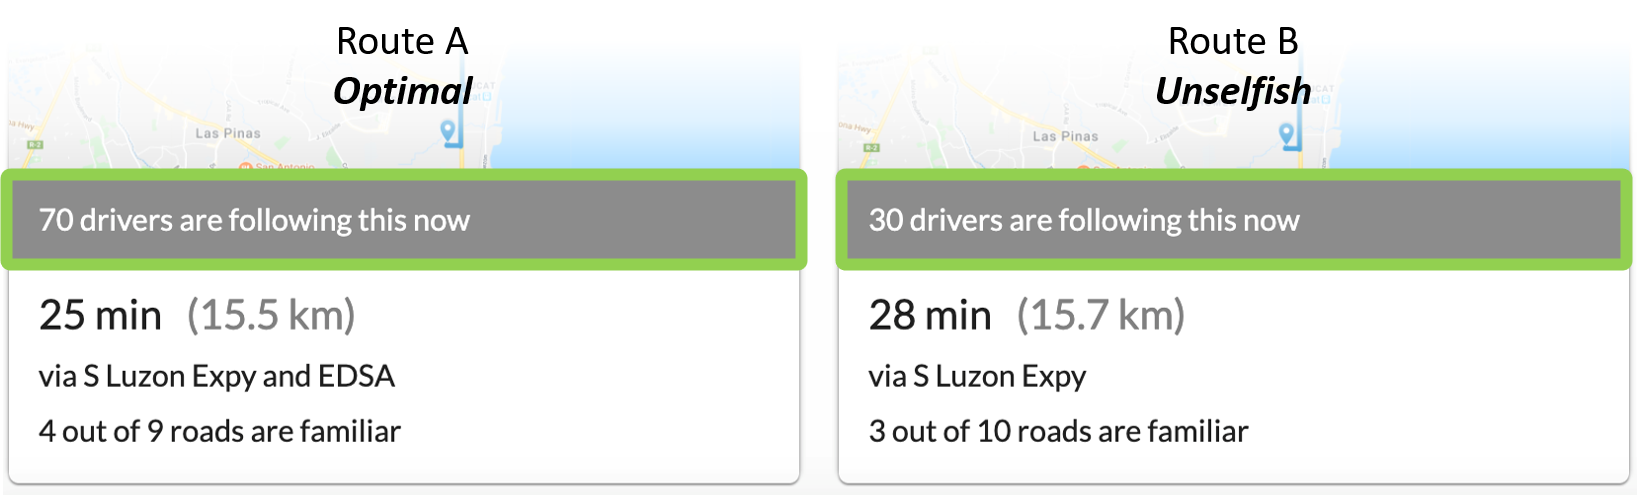
\includegraphics[scale=0.4]{figures/s3-critimass.png}
  \caption{The critical mass information shown for the optimal and unselfish routes. Because of induced demand brought about by a faster travel time, the number of drivers shown in the optimal route (left) is relatively more than the number of drivers taking the unselfish route.}~\label{fig:s3-critmass}
\end{figure}

To address the need for relatedness, critical mass information was used to show a hypothetical number of drivers that are currently taking the recommended route (Figure \ref{fig:s3-critmass}). This follows technique 4 (Information provision of other's behavior) from the CALO-RE taxonomy\cite{michie2011refined} and code 6.2 (Social Comparison) of BCT Taxonomy V1\cite{michie2013behavior}. The technique aims to show information about what others typically do with regards to the target behavior. 

In psychology, critical mass is used to regulate the belief that a large number of people are thinking or doing the same, and it is a common strategy to produce collective action\cite{oliver1985theory}. In this study, instead of highlighting that there are many drivers currently taking a route (something that should be avoided because of traffic congestion), critical mass information was used to emphasize that there are less people taking the unselfish route. I hypothesize that by seeing this information, drivers would be encouraged by the low number and discouraged by the high number for the optimal route. To maintain the sense of autonomy and control for the user, and reduce social desirability bias, both route choices showed a critical mass number.

\subsection{Valence}

\begin{figure}[h]
\centering
  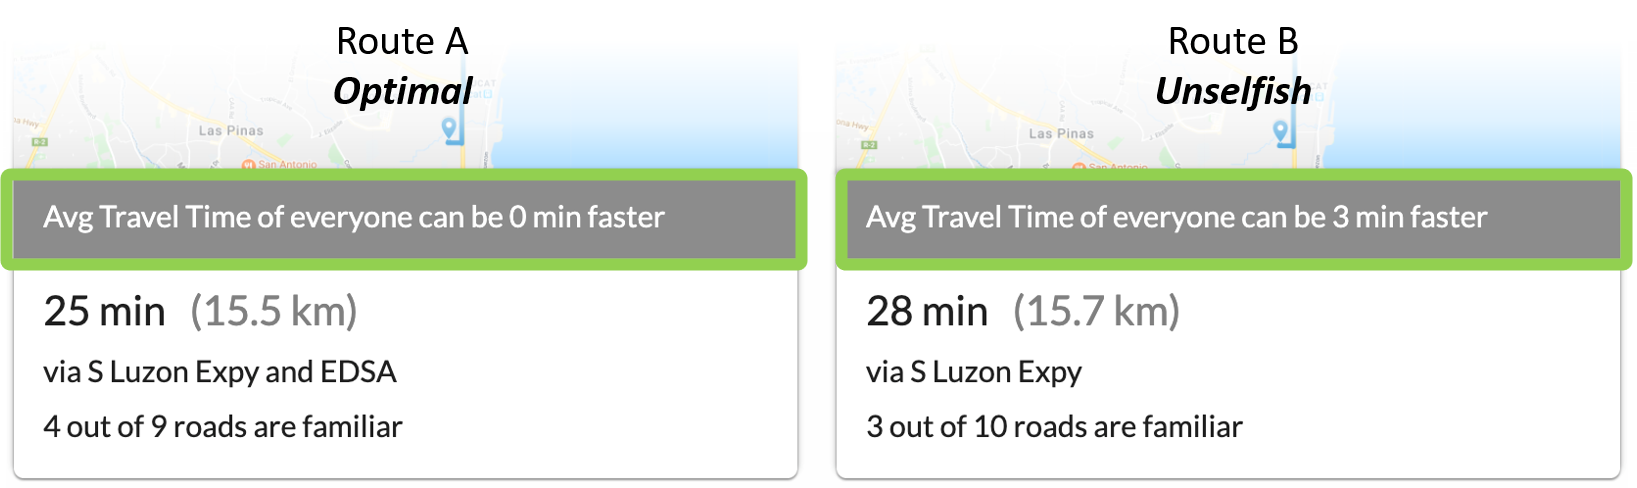
\includegraphics[scale=0.4]{figures/s3-valence.png}
  \caption{The valence information shown for the optimal and unselfish routes. For both route choices, it shows the estimated average travel time of all active drivers after the user makes a choice.}~\label{fig:s3-valence}
\end{figure}

Another popular strategy into convincing people to choose between options is by highlighting differences between them. In the context of driving, these could be differences in travel time or total distance. This follows techniques 1 (Information provision - general) and 2 (Information provision to the individual) from the CALO-RE taxonomy\cite{michie2011refined} and code 5.2 (Salience of consequences) of BCT Taxonomy V1\cite{michie2013behavior}. The technique aims to ``emphasize the consequences of performing the behaviour with the aim of making them more memorable,''\cite{michie2013behavior} both for the individual and in a general sense. 

Recently, Ringhand \& Vollrath\cite{ringhand2019faster} found that routes that positively frame travel time gains were chosen more than the way drivers avoided routes with negatively framed travel time loses. Here, gain or valence framing was used to highlight the amount of travel time that drivers can hypothetically and potentially win back if they choose a certain route. The optimal route always show a 0 minute gain because it only benefits an individual driver. But theoretically, there might be a loss in travel time especially when it actually leads to traffic congestion. On the other hand, varying gains for the unselfish route was shown depending on the type of trip and recommended routes. For example in Figuree \ref{fig:s3-valence}, if the optimal route will take 25 minutes and choosing the unselfish route will take 28 minutes, it will be shown that the driver can experience a 3 minute gain if they choose the unselfish route. This number is the difference between the two travel times. This means that if a driver cooperates with everyone and follows a sub-optimal unselfish route, they can actually reduce their travel time and still arrive at their destination with the same travel time as the optimal route. The phrase \textit{``\textit{Avg Travel Time of everyone can be...}''} was used to denote uncertainty because we cannot expect that everyone will follow their unselfish routes. In here, we deliberately emphasized the uncertainty of this information to give the ultimate decision on the driver and not give authoritative numbers that they might regret not following later. 

\subsection{Simple Positive Framing}

\begin{figure}[h]
\centering
  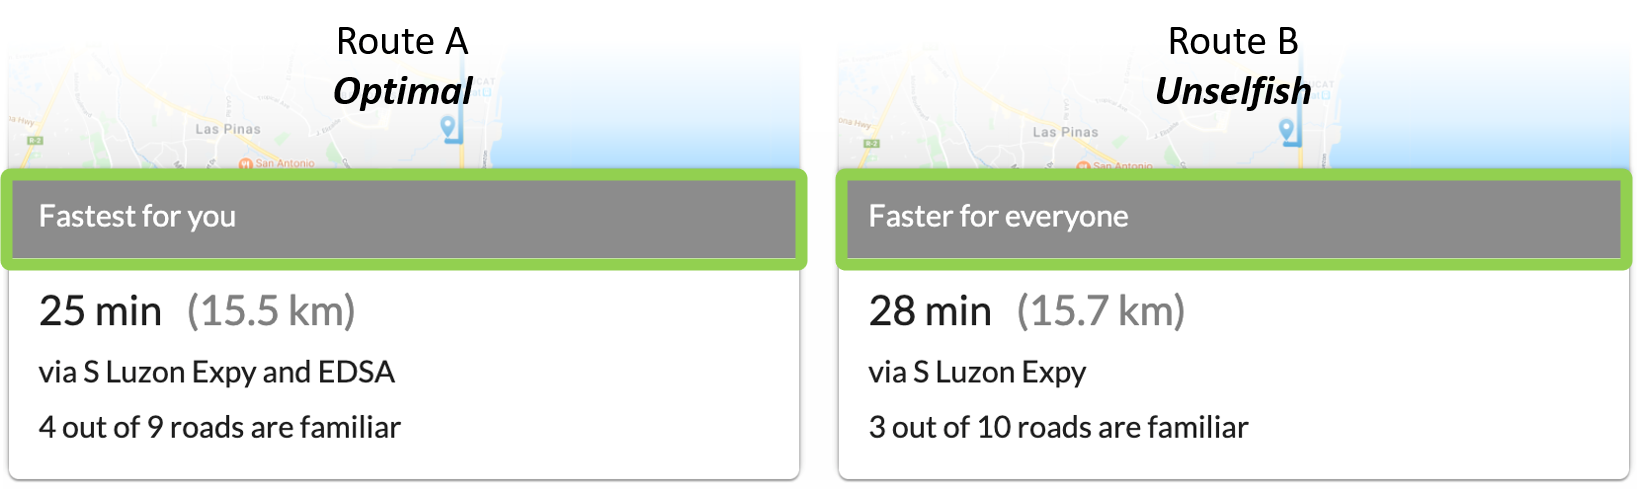
\includegraphics[scale=0.4]{figures/s3-framing.png}
  \caption{The navigational information that uses simple positive framing of the consequences of choosing a certain route.}~\label{fig:s3-framing}
\end{figure}

The last motivative information is the simple positive framing of the kinds of benefit drivers might experience by following either routes. Similar to the valence information, this also follows techniques 1 (Information provision - general) and 2 (Information provision to the individual) from the CALO-RE taxonomy\cite{michie2011refined} and code 5.2 (Salience of consequences) of BCT Taxonomy V1\cite{michie2013behavior}. Again, the goal is to ``emphasize the consequences of performing the behaviour with the aim of making them more memorable,''\cite{michie2013behavior} both for the individual and in a general sense. But unlike the previous technique of showing quantitative values, this technique focuses on using qualitative information to convince drivers.

Currently, Waze puts an \textit{``Optimal''} label with its top recommendation while Google Maps uses the phrases that read like \textit{``Fastest route, lighter traffic than usual.''} Instead of those leading labels and using ``Unselfish'' for the sub-optimal route, I opted for phrases that does not overemphasize one recommendation over the other (Figure \ref{fig:s3-framing}). While it is a typical technique to nudge drivers into choosing a desired route, which in this case is the unselfish one, I also want to give the impression that there is no wrong choice between Route A and B. Whichever they choose, someone or everyone will eventually benefit, and we are leaving that for them to decide. The pronouns \textit{``you''} and \textit{``everyone''} were used to indicate the main beneficiaries of the choice. 

\section{Familiarity Information}

\begin{figure}[h]
\centering
  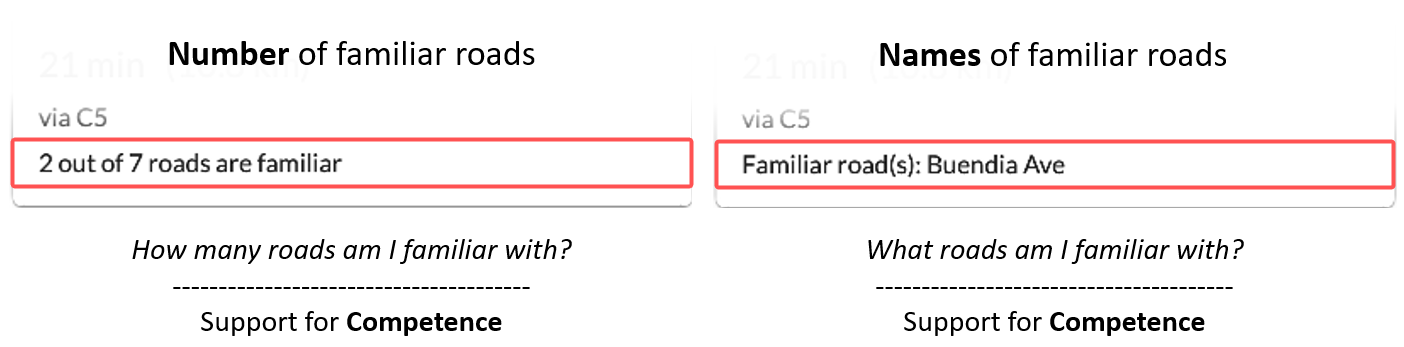
\includegraphics[scale=0.6]{figures/s3-familiarity.png}
  \caption{The two types of road familiarity information shown to drivers for both route choices. The left version shows the number of distinct roads that are familiar, while the right version shows the exact names of some familiar roads.}~\label{fig:s3-familiarity}
\end{figure}

Aside from benefits in travel time, drivers exhibit strong bias towards routes that are familiar to them\cite{Samson:2019:EFI:3290605.3300601,Patel2006PersonalizingRoutes}. In current navigation applications, the name of a major road is typically shown along with the travel time and total distance. Given that unselfish routes are relatively sub-optimal, I hypothesize that adding information about the roads that are familiar to them will increase their motivation to make the unselfish choice. Figure \ref{fig:s3-familiarity} shows the two types of familiarity information. The first one shows the number of familiar roads out of the total number of distinct roads in the route. The second lists up two names of familiar roads. Both information supports the need for autonomy and competence. 

In the prototypes used in this study, the number of familiar roads was based on the number of unique roads in the route that the participant has recalled to be familiar with. The total number of unique roads in the recommended route is also shown along with it. 

For the \textit{Name of familiar roads} information, at most two road names was shown at a time. If the participant is familiar with more than 1 road along the route, we will show the familiar road that is not shown as a major road according to Google Map results. If there is only 1 familiar road and it is the same as the major road(s) returned by Google Maps, then we will just repeat that information.

The familiarity information was gathered from the preliminary survey where participants are asked to list down all roads that they can possibly recall. In practice, there might be more roads that a driver knows. 

\section{Method}
This study focuses on investigating the effects of adding motivative and familiarity information to the route choice of drivers. In particular, I want to investigate if adding motivative and familiarity information will make drivers choose the unselfish route more, regardless of trip purpose. Additionally, I want to see if the stated choice for the unselfish route will be higher in non-commute trips. Thus, we conducted an online experiment with a 4x3x2 within-subject design. There were three types of independent variables, namely:
\begin{itemize}
    \item \textbf{Purpose of trip:} Work-to-home (\textbf{W2H}), home-to-work (\textbf{H2W}), work-to-frequent place (\textbf{W2F}) and home-to-frequent place (\textbf{H2F})
    \item \textbf{Motivative Info:} Critical mass (\textbf{C}), valence framing (\textbf{V}) and simple positive framing (\textbf{F})
    \item \textbf{Road Familiarity Info:} Number of familiar roads (\textbf{P}) and names of familiar roads (\textbf{R})
\end{itemize}

We added four (4) baseline conditions that show route choices for each purpose of trip but without any motivative or road familiarity information. In total, there are 28 experimental conditions that each participant will perform a task for. To avoid ordering effects, conditions were balanced using a Latin square.

\subsection{Participants}
We recruited 28 participants in multiple rounds. They were included in a lottery where one winner will receive a cash reward of 2,500 Japanese yen. They were recruited through snowball sampling. An initial call for participation was posted on two private groups on social media composed of people from academic institutions and alumni. As an inclusion criteria, we only recruited participants who are adults (18 to 60 y.o.), has an active or valid driver's license and drives to work, business or school on most days of the week (more than 3 times). They are comprised of people who identify as men (N=17), women (N=10) and non-binary (N=1). Their ages range between 21 to 52 years old (M=28). In terms of driving years, 2 are driving for less than a year, 12 for 1 to 5 years, 5 for 5 to 10 years, and 9 of them are driving for more than 10 years. Looking at driving experience, 6 participants have been driving for less than 15,000km, 11 have driven between 15,000km to 25,000km, and 11 have driven more than 25,000km. 

When asked about how often they switch between their regular and alternative routes, half of them (N=14) switch once a week when going to work or school. Six (6) of them do it twice or more in a week while 8 participants never switch to an alternate route. When going back home from school or work, half of them switch once a week while 8 are doing it twice or more. Six of them never switch. 

\subsection{Protocol}
Participants were tasked with answering a preliminary survey, an online experiment, and two post-hoc questionnaires (Figure \ref{fig:s3-protocol}). 

\begin{figure}[h]
\centering
  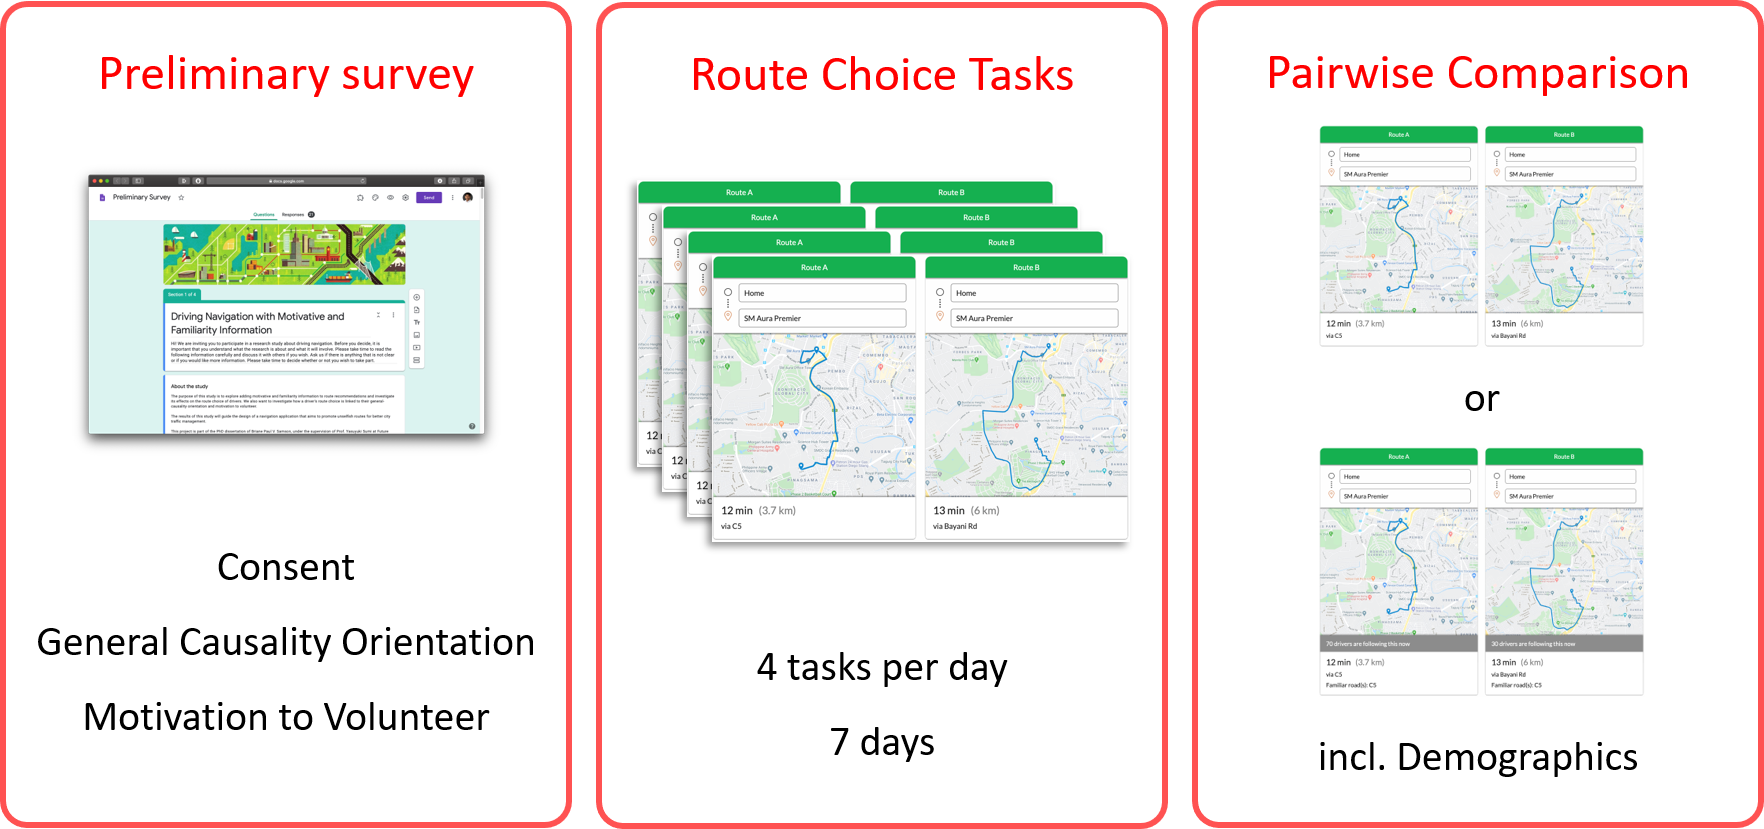
\includegraphics[scale=0.5]{figures/s3-protocol.png}
  \caption{An overview of the study protocol.}~\label{fig:s3-protocol}
\end{figure}

\subsubsection{Preliminary Survey}
The preliminary survey consists of four sections. The first section asks for their consent to participate, age, gender and driving experience. Because the online experiment will be administered through email, they were required to provide an email address. For those who do not check their emails regularly, they were given the option to provide their Facebook Messenger or Line details.

The second section asks about the places that they frequently drive to (home, work or school, and two frequently visited places) and roads they are familiar with (free text). They were also asked to find those locations on Google Maps and submit the URLs. Then in the third section, they are asked to complete the 12-item General Causality Orientations Scale (GCOS) which represent their orientation towards autonomy, relatedness, and competence. In the fourth and last section, they are asked to complete the 24-item Motivation to Volunteer Scale to learn about their behavioral regulatory styles according to SDT, and their recent experiences of volunteering. 

After submitting the preliminary survey, they were sent an introduction about the online experiment and on what to prepare and expect. The preliminary survey took approximately 25-30 minutes to complete. For full details, please refer to Appendix \ref{AppendixD}.

\subsubsection{Online Experiment}
The online experiment was divided into 7 questionnaires with 4 items each. They were sent daily to their emails at 10:00AM local time for 7 working days (Monday to Friday only). Their first questionnaires were sent at most two (2) days after they completed the preliminary survey form. This protocol was designed in order to avoid learning effect.

\begin{table}[h]
    \caption{The order of conditions for Participant 22 during the 7-day online experiment. The acronyms stand for the pair of motivative and familiarity information for that condition. For example, BL means baseline condition while FR represents the condition that uses simple positive framing (F) and shows the name of familiar roads (R).}
	\label{tab:sample-order}
	\centering
	\begin{tabular}{l c c c c}
	    \hline\hline
		& \textbf{W2H} & \textbf{H2W} & \textbf{W2F} & \textbf{H2F} \\
		\hline
		Day 1 & BL & CP & VR & VP \\
        Day 2 & FR & VP & CR & FP \\
        Day 3 & CR & BL & FR & CR \\
        Day 4 & FP & FP & FP & CP \\
        Day 5 & CP & FR & BL & BL \\
        Day 6 & VR & CR & VP & FR \\
        Day 7 & VP & VR & CP & VR \\
		\hline
	\end{tabular}
\end{table}

The daily questionnaire has 4 route choice scenarios which represent work-to-home (W2H), home-to-work (H2W), work-to-frequent (W2F) and home-to-frequent(H2F) trips, given in that order. To illustrate, Table \ref{tab:sample-order} shows the order of conditions for Participant 22 during the 7-day online experiment. Everything can be accomplished in less than 10 minutes. Each item in the questionnaire presents a navigation scenario and two images of the prototypical navigation app interfaces that show the recommended routes A and B (Figure \ref{fig:s3-daily-proto}). The map shown is not interactive and is only meant to give a visual representation of the route suggestions. Below the map is the set of navigational information which varies depending on the experimental condition.

\begin{figure}[h]
\centering
  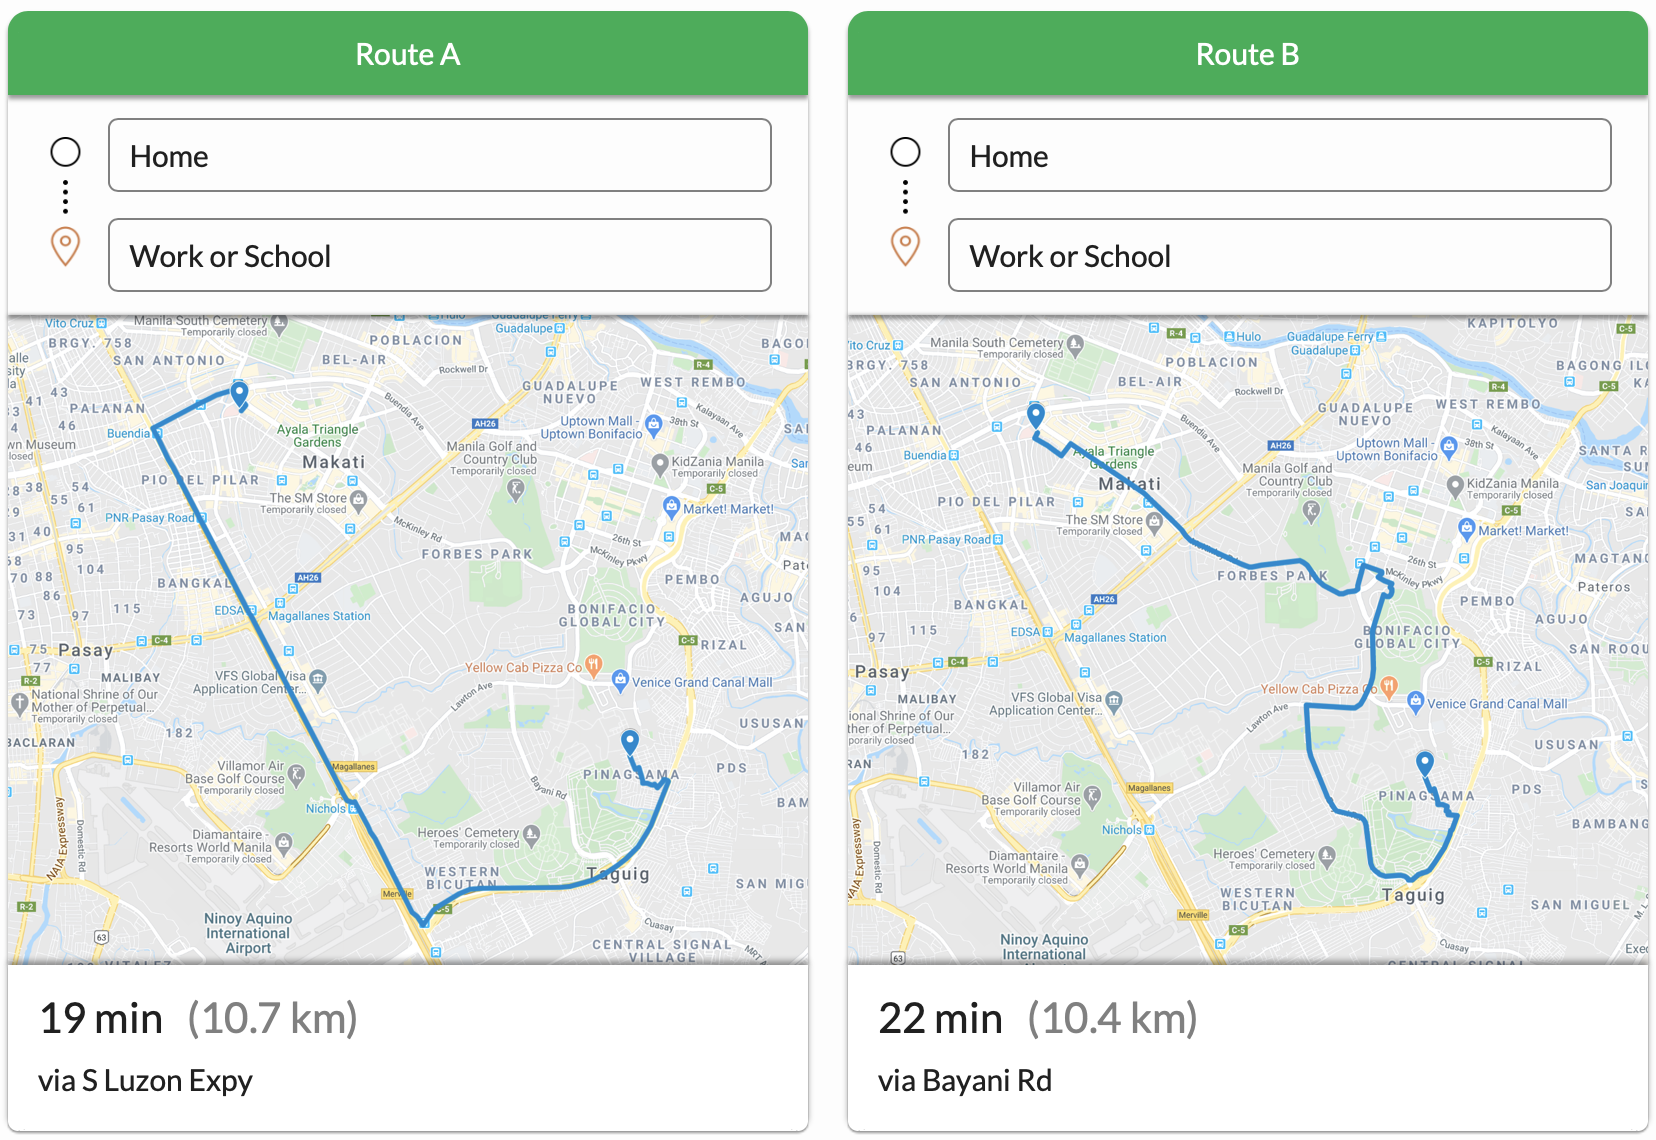
\includegraphics[scale=0.4]{figures/s3-daily-proto.png}
  \caption{The baseline (BL) version of the prototypical navigation app interface. Routes A and B are shown side-by-side. The top part shows the origin and destination with the map below it. The bottom part shows the navigational information that you would typically find in most navigation applications. This part has 27 other versions for each experimental condition.}~\label{fig:s3-daily-proto}
\end{figure}

Before answering the first route choice scenario, participants were asked prepare a timer or clock nearby. For each scenario, they were asked to record the amount of time it took them to make a choice. They were allowed to answer the questionnaire any time within the day but they have to be submitted before the day ends. Sample screenshots of the daily questionnaire can be seen in Appendix \ref{AppendixF}.

\subsubsection{Post-Hoc Questionnaires}
On their last day of the online experiment, they were given two post-hoc questionnaires along with the Day 7 questionnaire. The first questionnaire asks about their demographic and socioeconomic information, and driving experience. The second questionnaire ask them to make pairwise comparisons between the different experimental conditions used in the online experiment.  

\subsubsection{Interviews}
After all 28 participants are completed, we will send invitations for a short interview. I will ask about their qualitative feedback on the sets of motivative and familiarity information shown to them. They will also be presented with their most preferred condition after the pairwise comparison task and asked why they think that is the most convincing combination for them.

\section{Design}
The interface prototype mimics the typical design of most modern navigation applications in the market (e.g. Google Maps, Waze). The screen shows the origin and destination of the trip at the top and a map in the middle. The bottom of the screen shows the navigational information section, for which we created 7 versions. But for all versions of the navigational information section, it always contains the basic set of estimated travel time, total distance and name(s) of major roads. Figure \ref{fig:s3-daily-proto} shows the baseline (BL) version that features the basic set of information. For the six other versions, new information are added on top and bottom parts of the navigational information section. In Figure \ref{fig:s3-navi-parts}, the motivative information is added on the gray box at the top and the familiarity information is added below the name of a major road. Both use the same font size to reduce bias in visual hierarchy. Figure \ref{fig:s3-versions} shows all six versions for each combination.

\begin{figure}[h]
\centering
  
\includegraphics[scale=.8]{figures/s3-navi-parts.png}
  \caption{The additional parts of the navigational information section for the 6 treatment conditions.}~\label{fig:s3-navi-parts}
\end{figure}

\begin{figure}[h]
\centering
  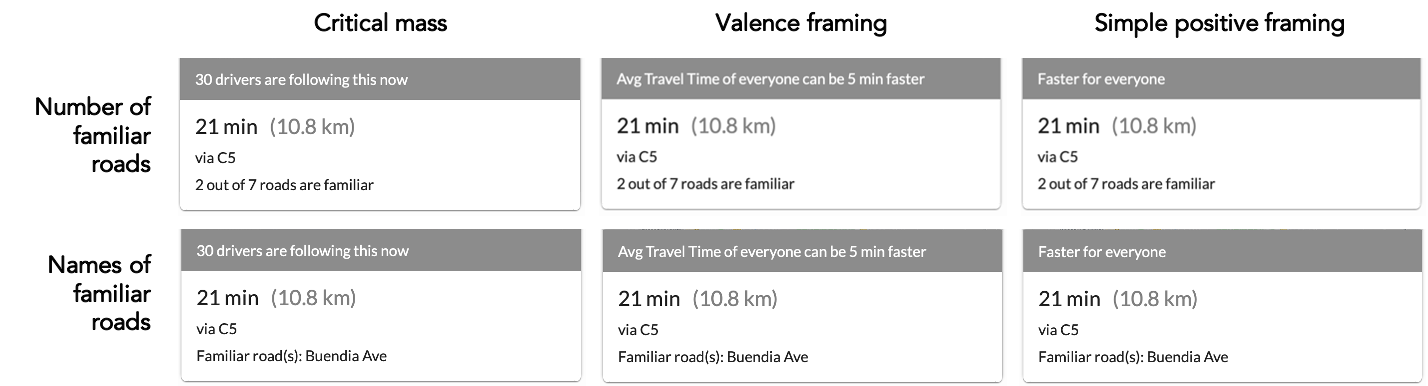
\includegraphics[scale=0.55]{figures/s3-versions.png}
  \caption{The design versions of the navigational information section that adds different combinations of motivative and familiarity information. The versions aligned in the same column use the same motivative information. For example, the two versions in the leftmost column both show critical mass (C) information. The versions in the same row use the same familiarity information.}~\label{fig:s3-versions}
\end{figure}

\section{Materials and Measures}
Because of the remote nature of this study, the participants were asked to answer a number of questionnaires using Google Forms.

\subsection{Measuring Motivation}
We are also interested in understanding whether our autonomy-supportive motivative information are effective in promoting the unselfish route for different regulatory styles and causality orientations. We used two standard questionnaires to measure motivation based on SDT constructs. 

The General Causality Orientation Scale (GCOS)\cite{Deci1985GCOS} measures people's causality orientations on three sub-scales, namely autonomy, control and impersonal. We used the standard 12-item vignette and followed the recommended scales and ordering. Each question presents a scenario with three possible responses. Participants are asked to rate on a scale of 1 to 7 the likelihood that they will respond to the given situation in a certain way. 

On the other hand, the Motivation to Volunteer Scale (MVS)\cite{grano2008motives} measures a person's volunteering motivation based on 24 items. Each of the 6 behavior regulatory styles is represented by 4 items. Participants were asked to what extent do each item correspond to their personal motives for engaging in volunteering. They gave ratings on a scale of 1 (does not correspond at all) to 5 (corresponds exactly). Items were randomized to avoid ordering effect. Because the MVS questionnaire is relatively long, we also added an attention check item. At the end of the preliminary survey, we also asked them about their volunteering experience: ``How often have you participated in volunteering activities in the past three months on average?'' Because the COVID-19 pandemic has unexpectedly motivated people to volunteer, we asked a second question ``How often have you participated in volunteering activities on average from October to December 2019 (before COVID-19 pandemic)?'' for them recall their volunteering frequency before the pandemic and to check for consistency with the first question. Both questions were answered using three options: Never, Once a week and Twice a week or more.

For both GCOS and MVS, we will compute the mean score per sub-scale and use it in the analysis.

\subsection{Route Recommendations}
The route recommendations used in the questionnaires were personalized for each participant using the information they provided from the preliminary survey. For each type of trip, we searched for the fastest route and a sub-optimal route using Google Maps. Searches were done during mid-day to maintain consistency across participants. The fastest route is the route recommendation with the shortest travel time while the sub-optimal route is the recommendation with the longest distance and or longer travel time. The sub-optimal route was used as the unselfish route and assigned as Route B. Route A is always the fastest. To prepare the maps used in the prototypes, we traced the recommended routes using Google My Maps. 

For each participant, a total of 8 route recommendations were prepared. 

\subsection{Stated Route Choice}
The daily route choice questionnaires contain 4 binary route choice tasks. They were instructed that they will be making 4 independent trips: 
\begin{itemize}
    \item Work/School to Home
    \item Home to Work/School
    \item Work/School to a frequently visited place
    \item Home to a frequently visited place 
\end{itemize}

Before seeing the prototypes, they were asked to imagine the following scenario:
\begin{quote}
    In each trip, imagine that you are just about to leave and go to a destination. Before leaving your point of origin, you bring out your smartphone and open a navigation application. You are not driving yet. You type your destination in the navigation application and search for routes. Two route suggestions are shown and you have to choose which one to follow. For all route suggestions, you are shown a static map of the route, the estimated travel time, distance and a major road included in the route. Assume that these navigational information are reliable and that you will arrive at your destination on time regardless of choice. 
\end{quote}

Participants were also asked to imagine that a hypothetical Traffic Management System is active during the trips using the following prompt:
\begin{quote}
    Imagine that your city has implemented a Traffic Management System (TMS) to help optimize the traffic flow on its roads. It is run by the city government and receives constant traffic updates in order to make proper traffic assessments. Assume that the information they collect and use are reliable. Its goal is to equally distribute active cars in the road network so that everyone benefits. In order to achieve this, it gives recommendations to connected drivers. However, it does not always distribute drivers to optimize traffic flow. It only happens when they anticipate that many drivers will start using the roads. 

    Your navigation application is connected to this system and it adjusts the route suggestions based on what the TMS recommends. When it predicts that traffic congestion will occur or has already happened, it will now recommend a route that will help ease traffic flow in other areas, along with the usual recommendation of the fastest route. The route suggestions may include 2 types of additional information to help you with your route choice. The first type of information describes how the route can contribute to everyone's travel time. The second information describes how familiar it is to you. You are free to accept or ignore the recommendations and additional information. You will not receive any penalty. 

    In all of the trips, assume that the TMS is detecting traffic congestion on some roads. The traffic flow is now being distributed and you are part of it.
\end{quote}

After reading the scenarios, participants were asked to prepared a timer. The following sections of the questionnaire gave the 4 route choice tasks. Participants were asked to choose between Route A and B. They were also asked to time their decision making from the moment they saw the prototypes up to the time they selected their final choice.

\subsection{Pairwise Comparison}
On top of recording their stated preferences after seeing different types of navigational information, I also wanted to measure their relative preferences using pairwise comparison. For this, I only used the prototypes for the home-to-work trips. Participants were asked to compare 21 pairs of the 7 design versions that were randomly ordered. One (1) item was repeated to act as attention check and to check for consistency of answers. In total, there were 22 pairwise comparisons made. Sample screenshots of the questionnaire can be seen in Appendix \ref{AppendixE}.

\section{Results}
I begin the discussion of results with the analysis of their stated route choice in the online experiment. Lastly, I present the results of the pairwise comparison task. 

\subsection{Causality Orientation and Motivation to Volunteer}
A Shapiro-Wilk normality test suggests that all sub-scale scores for both causality orientation and motivation to volunteer are normally distributed except for the Control sub-scale of causality orientation. In terms of data symmetry, only the GCOS Impersonal sub-scale scores were nearly symmetrical with a skewness of 0.06. The GCOS Control and the MVS Introjected, External and Amotivation sub-scales are right-skewed, in which their means are larger than their medians and have larger right-handed tails. The rest of the sub-scales are left-skewed. 

For the purpose of my analysis, the scores were binned into low, moderate and high categories. GCOS sub-scale scores less than 3 are considered low while those greater than 5 are considered high. Scores that fall between 3 and 5 are moderate scores. As for MVS sub-scale scores, those below 3 are also considered low, while those above 3 are coded as high. MVS sub-scale scores that are exactly 3 are considered moderate.

In terms of causality orientation, most of the participants scored highest on the Autonomy sub-scale ($\mu$ =  6.02, M = 6.08, $\sigma$ = 0.55) with 2 moderate scores and 26 high scores. All participants scored moderately (N = 27) in the Control sub-scale ($\mu$ =  4.18, M = 4.25, $\sigma$ = 0.69) except for one outlier that had a high score. Expectedly, the Impersonal sub-scale scores are relatively lowest but more diverse ($\mu$ =  3.587, M = 3.585, $\sigma$ = 0.98) with more than half of the participants having moderate scores (N = 18) while 8 of them are low. All of these suggests that our participant pool are mainly oriented towards environments or tools that provide informational feedback and allow choice, where they can have greater agency and intrinsic motivation. Their low Impersonal orientation suggests they believe that their desired outcomes can be attained, not just by luck or fate. Even so, they still show moderate tendency to be controlled by rewards, structure and the directives of others in order to perform tasks.  

In terms of behavioral regulation, the Motivation to Volunteer Survey  gave scores to the different styles according to SDT. Most of the participants scored high in the Intrinsic motivation ($\mu$ =  3.85, M = 4, $\sigma$ = 0.89), Integrated ($\mu$ =  3.25, M = 3.13, $\sigma$ = 0.94) and Identified ($\mu$ =  4.05, M = 4.13, $\sigma$ = 0.59) sub-scales. On the other hand, they scored low in the Introjected ($\mu$ =  2.44, M = 2.5, $\sigma$ = 0.82), External ($\mu$ =  2.08, M = 2.13, $\sigma$ = 0.77) and Amotivation ($\mu$ =  1.96, M = 2, $\sigma$ = 0.82) sub-scales. A Pearson correlation test suggests that the Intrinsic, Integrated and Identified sub-scale scores are more positively correlated as they are adjacent in the self-determined continuum. The same positive correlation was observed for the adjacent Introjected and External sub-scale scores. These are consistent with the Self-Determination Theory which posits that adjacent regulatory styles in the continuum are more associated with each other than those farther away\cite{ryan1989perceived}. Similar to Standage et. al. (2008)\cite{standage2008does}, the Intrinsic, Integrated and Identified sub-scale scores were averaged to have a score for autonomous motivation ($\mu$ =  3.72, M = 3.71, $\sigma$ = 0.6), while the Introjected and External scores were averaged to form the controlled motivation score ($\mu$ =  2.26, M = 2.19, $\sigma$ = 0.73). These results suggest that the participant pool has a stronger quality of intrinsic motivation towards volunteering and that they have a more internal perceived locus of causality. 

When asked about the average frequency of their volunteering activities for the past 3 months, twelve participants reported to have done some form of volunteer work at least once or more. Considering that the ongoing global pandemic have inspired people to volunteer more than they used to, we asked them about their average frequency of volunteer work between October to December 2019. They reported the same frequency. 

Combining the insights from the causality orientation and behavioral regulation scores, it suggests that the recruited participants would be more receptive to the proposed designs as they are intended to be autonomy-supportive. 

\subsection{Stated Route Choice}
From the results of the 7-day route choice task, I first investigate how often the unselfish route was chosen compared to the optimal one. Then, a Generalized Estimating Equations (GEE) model was created to estimate the population average effects and investigate the likelihood that the population will change their route choice given a pair of motivative and familiarity information. 

\subsubsection{Choice of Unselfish Route}

\begin{figure}[h]
\centering
  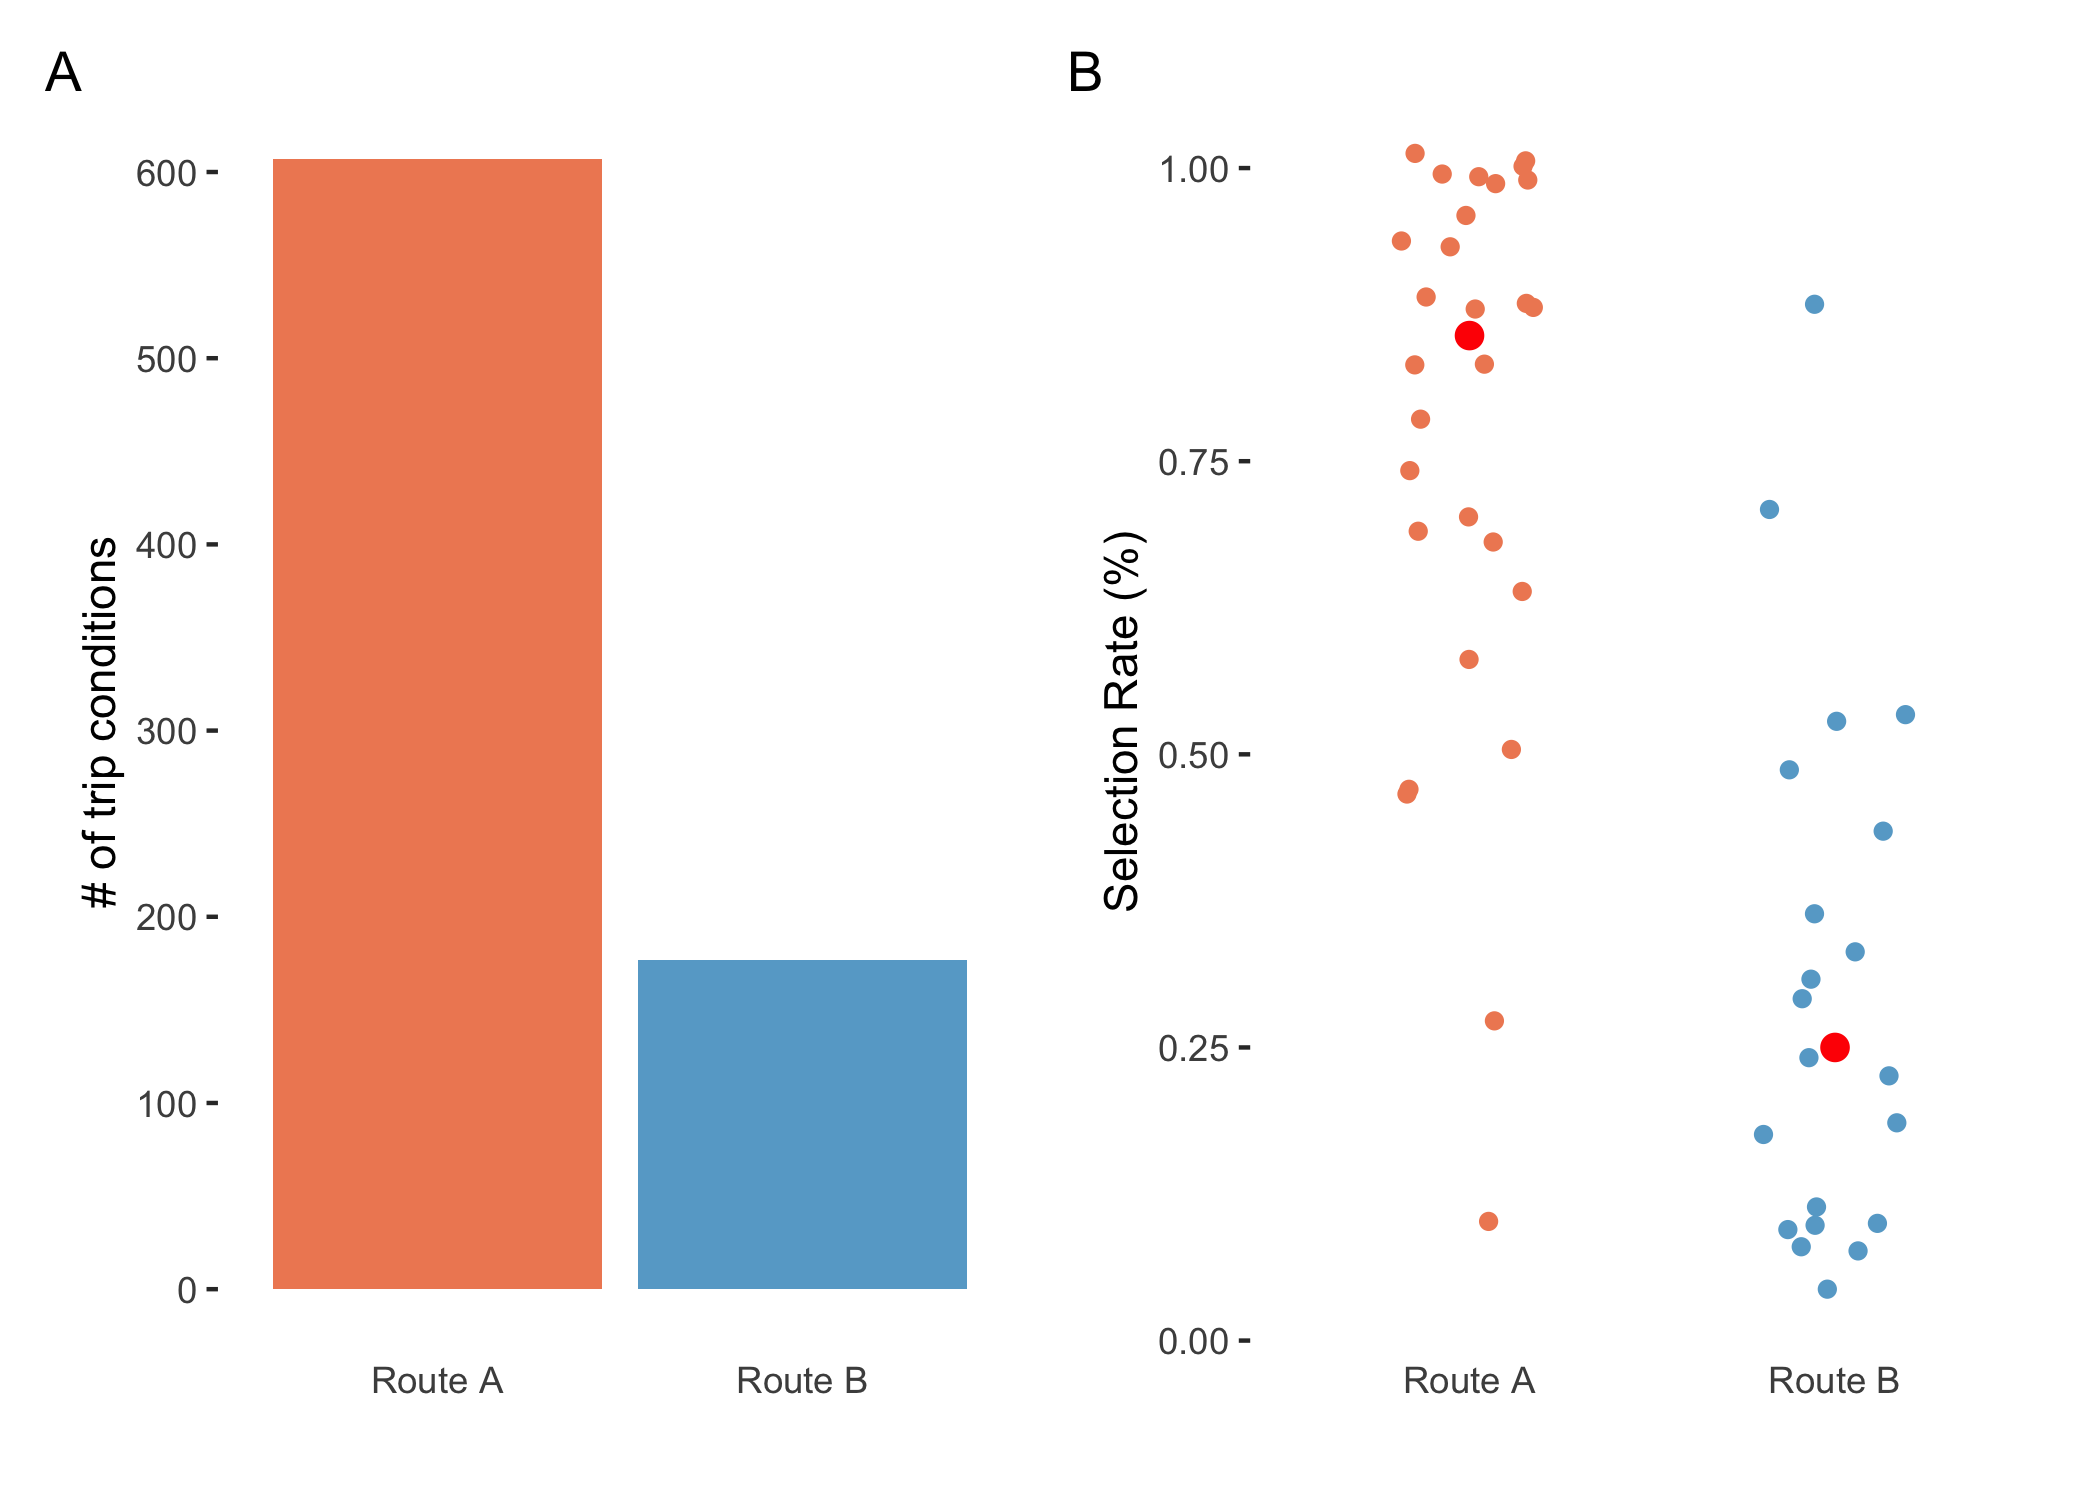
\includegraphics[scale=.2]{figures/s3-rc-all.png}
  \caption{A) The absolute number of trip conditions in which the participant chose each route. B) The rate by which each participant selected Routes A and B. The red dot shows the median selection rate.}~\label{fig:s3-rc-all}
\end{figure}

In absolute numbers, the unselfish route (Route B) was chosen in 177 (22.6\%) out of 784 trip conditions answered by all participants (Figure \ref{fig:s3-rc-all}A). Many participants (N=21) chose it at least once with a median selection rate of 25\% ($\mu$ =  0.301). The lowest rate is at 3.6\% (once) while the highest is at 89.3\% or around 24 times (Figure \ref{fig:s3-rc-all}B). Seven (7) participants never chose the unselfish route at all. 

\begin{figure}[h]
\centering
  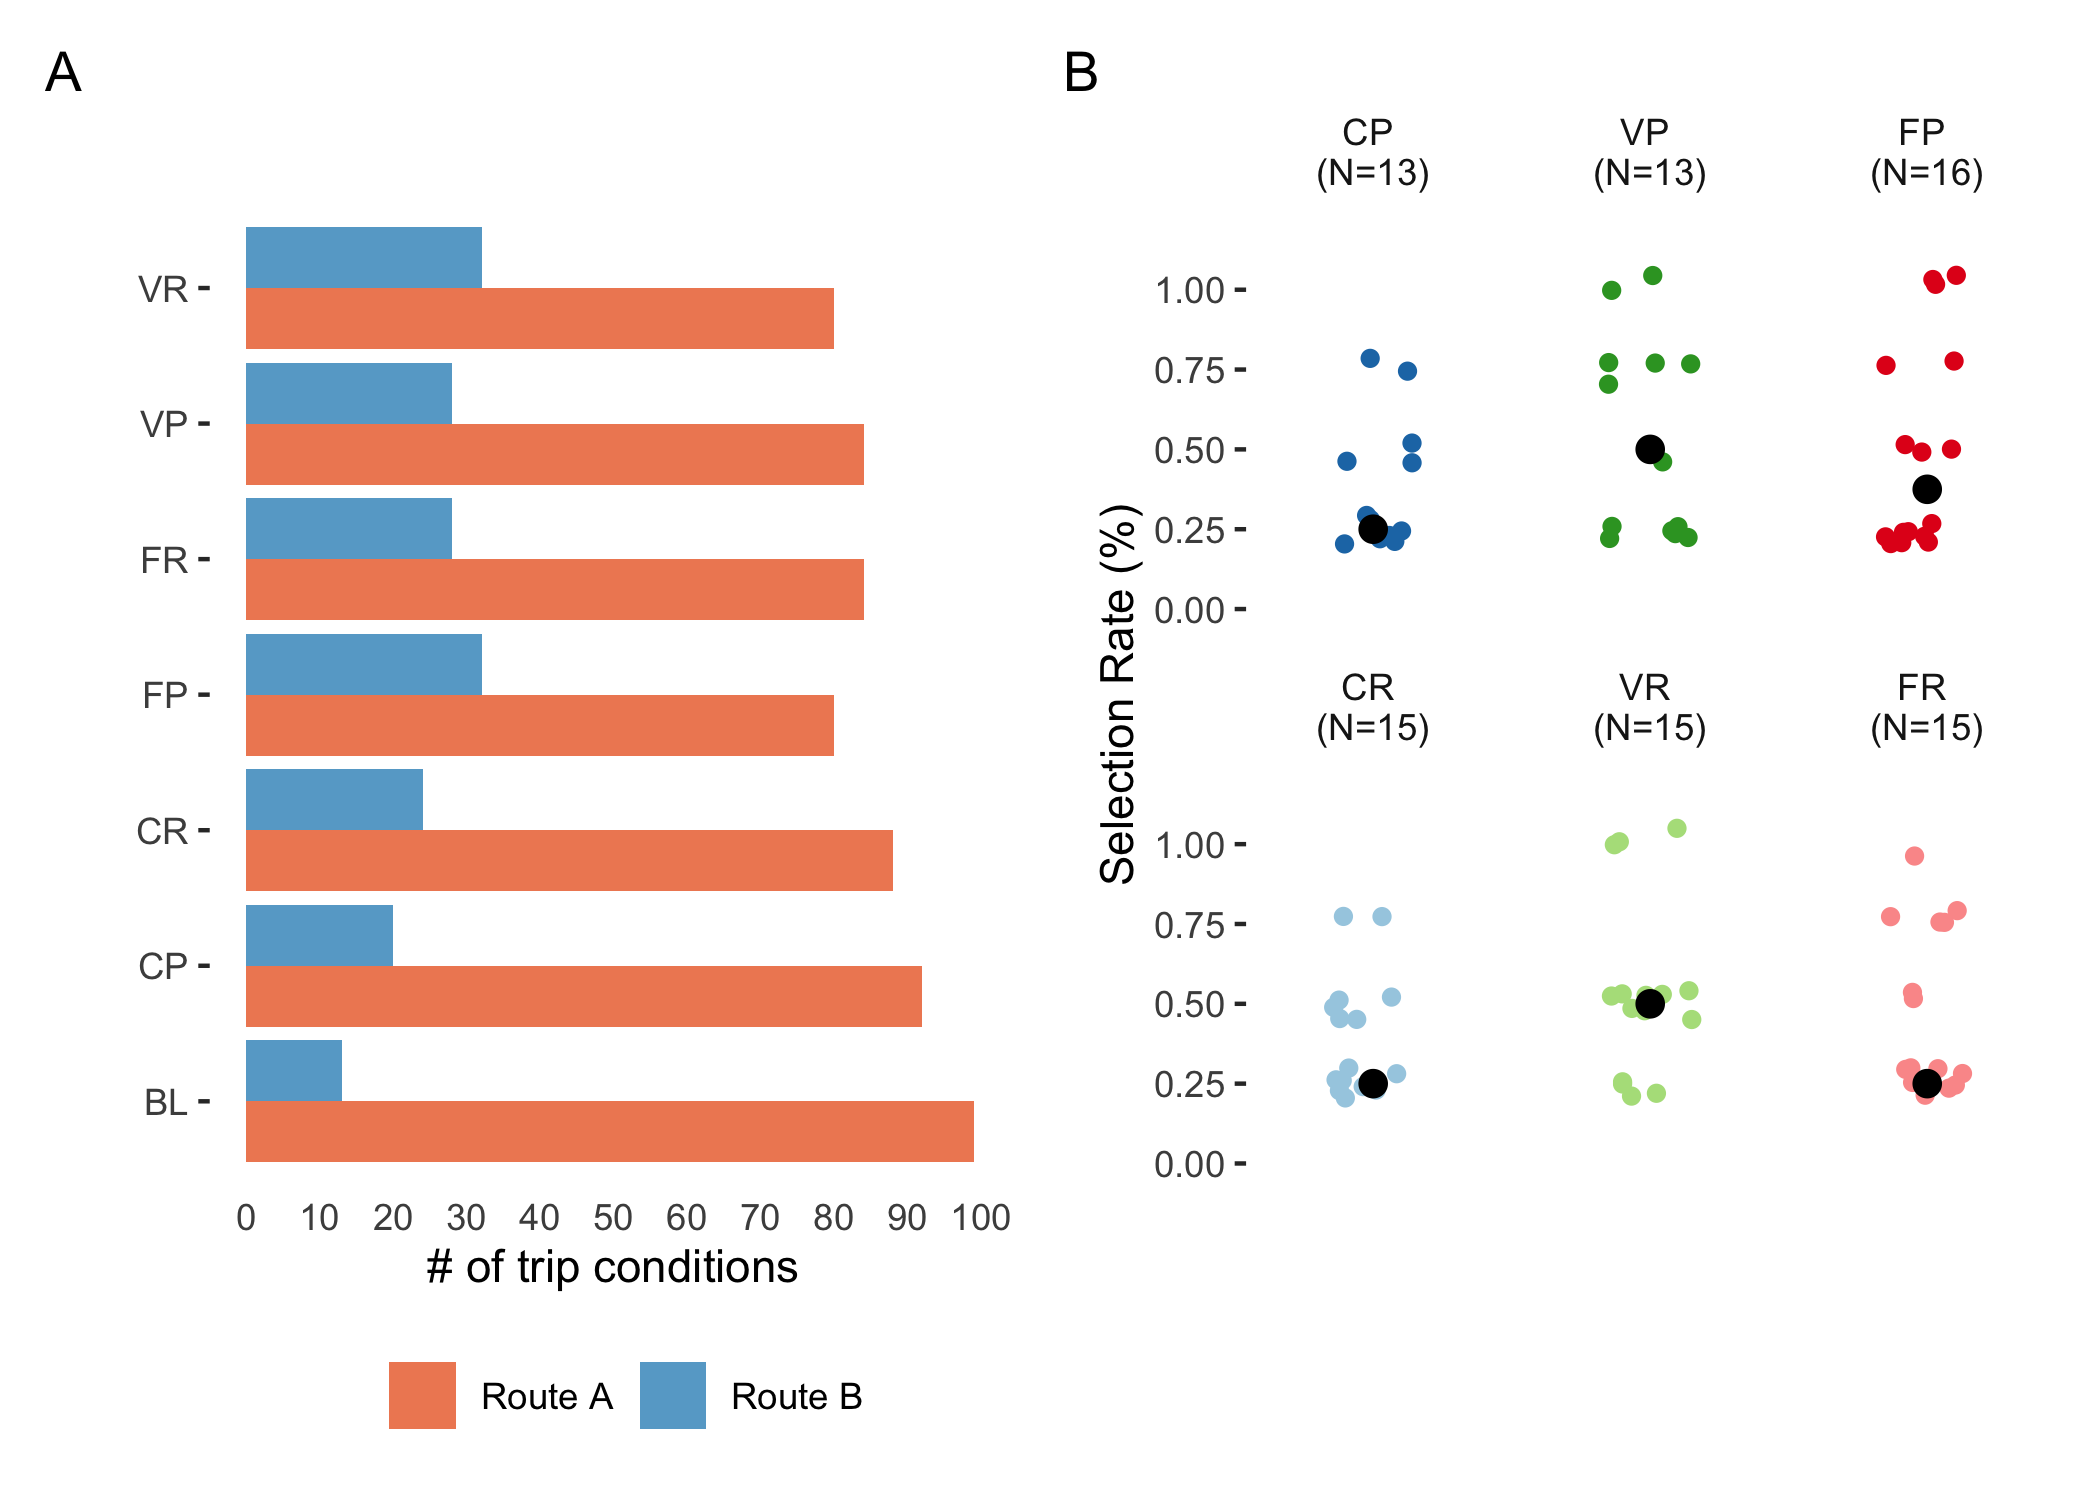
\includegraphics[scale=.2]{figures/s3-rc-unselfishratebycond.png}
  \caption{A) The number of trip conditions in which the participant chose each route and distributed by the combination of motivative and familiarity information. B) The rate by which participants selected Route B per combination. The black dot shows the median selection rate.}~\label{fig:s3-rc-unselfishratebycond}
\end{figure}

For the baseline (BL) condition in which no motivative and familiarity information is shown, the unselfish route was selected by six (6) participants at least once. Two of them selected Route B in all four (4) trip scenarios. Notably, they have also reported high autonomous orientation and high autonomous motivation. When they are shown the different combination of motivative and familiarity information, the number of times that Route B is selected relatively increases (Figure \ref{fig:s3-rc-unselfishratebycond}A). The most number of Route B selections happened when the \textbf{VR} (N=32) and \textbf{FP} (N=32) design versions were shown. Among the three (3) motivative information, participants chose the unselfish route the most when either the simple positive framing (N=60) or the valence information (N=60) was shown. This suggests that motivative information which explicitly highlights potential benefits of a future decision can positively impact the chance of selecting the unselfish route. On the other hand, the versions that showed the critical mass information (\textbf{CP} and \textbf{CR}) might have given a different impression which resulted to less instances of Route B being selected. 

Looking at the selection rate of each participant, the \textbf{FP} design version had the most number of participants (N=16) that selected Route B at least once in the four (4) trip scenarios. This is followed by all design versions that show the list of familiar roads (\textbf{CR}, \textbf{VR} and \textbf{FR}) with 15 participants selecting Route B at least once. Overall, participants had the highest selection rates when they were shown the \textbf{VP} ($\mu$ =  0.538, M = 0.5) and \textbf{VR} ($\mu$ =  0.533, M = 0.5) design versions. These results are indicative that if we want more drivers to adopt an unselfish route but with some inconsistency, we can focus on presenting them with information about the positive effects of choosing an unselfish route and or showing them the list of familiar roads. On the other hand, if we want drivers to be more consistent in choosing the unselfish route regardless of the trip scenario or type, the positive gain (i.e. decrease in travel time) should be explicitly shown. 

\begin{figure}[h]
\centering
  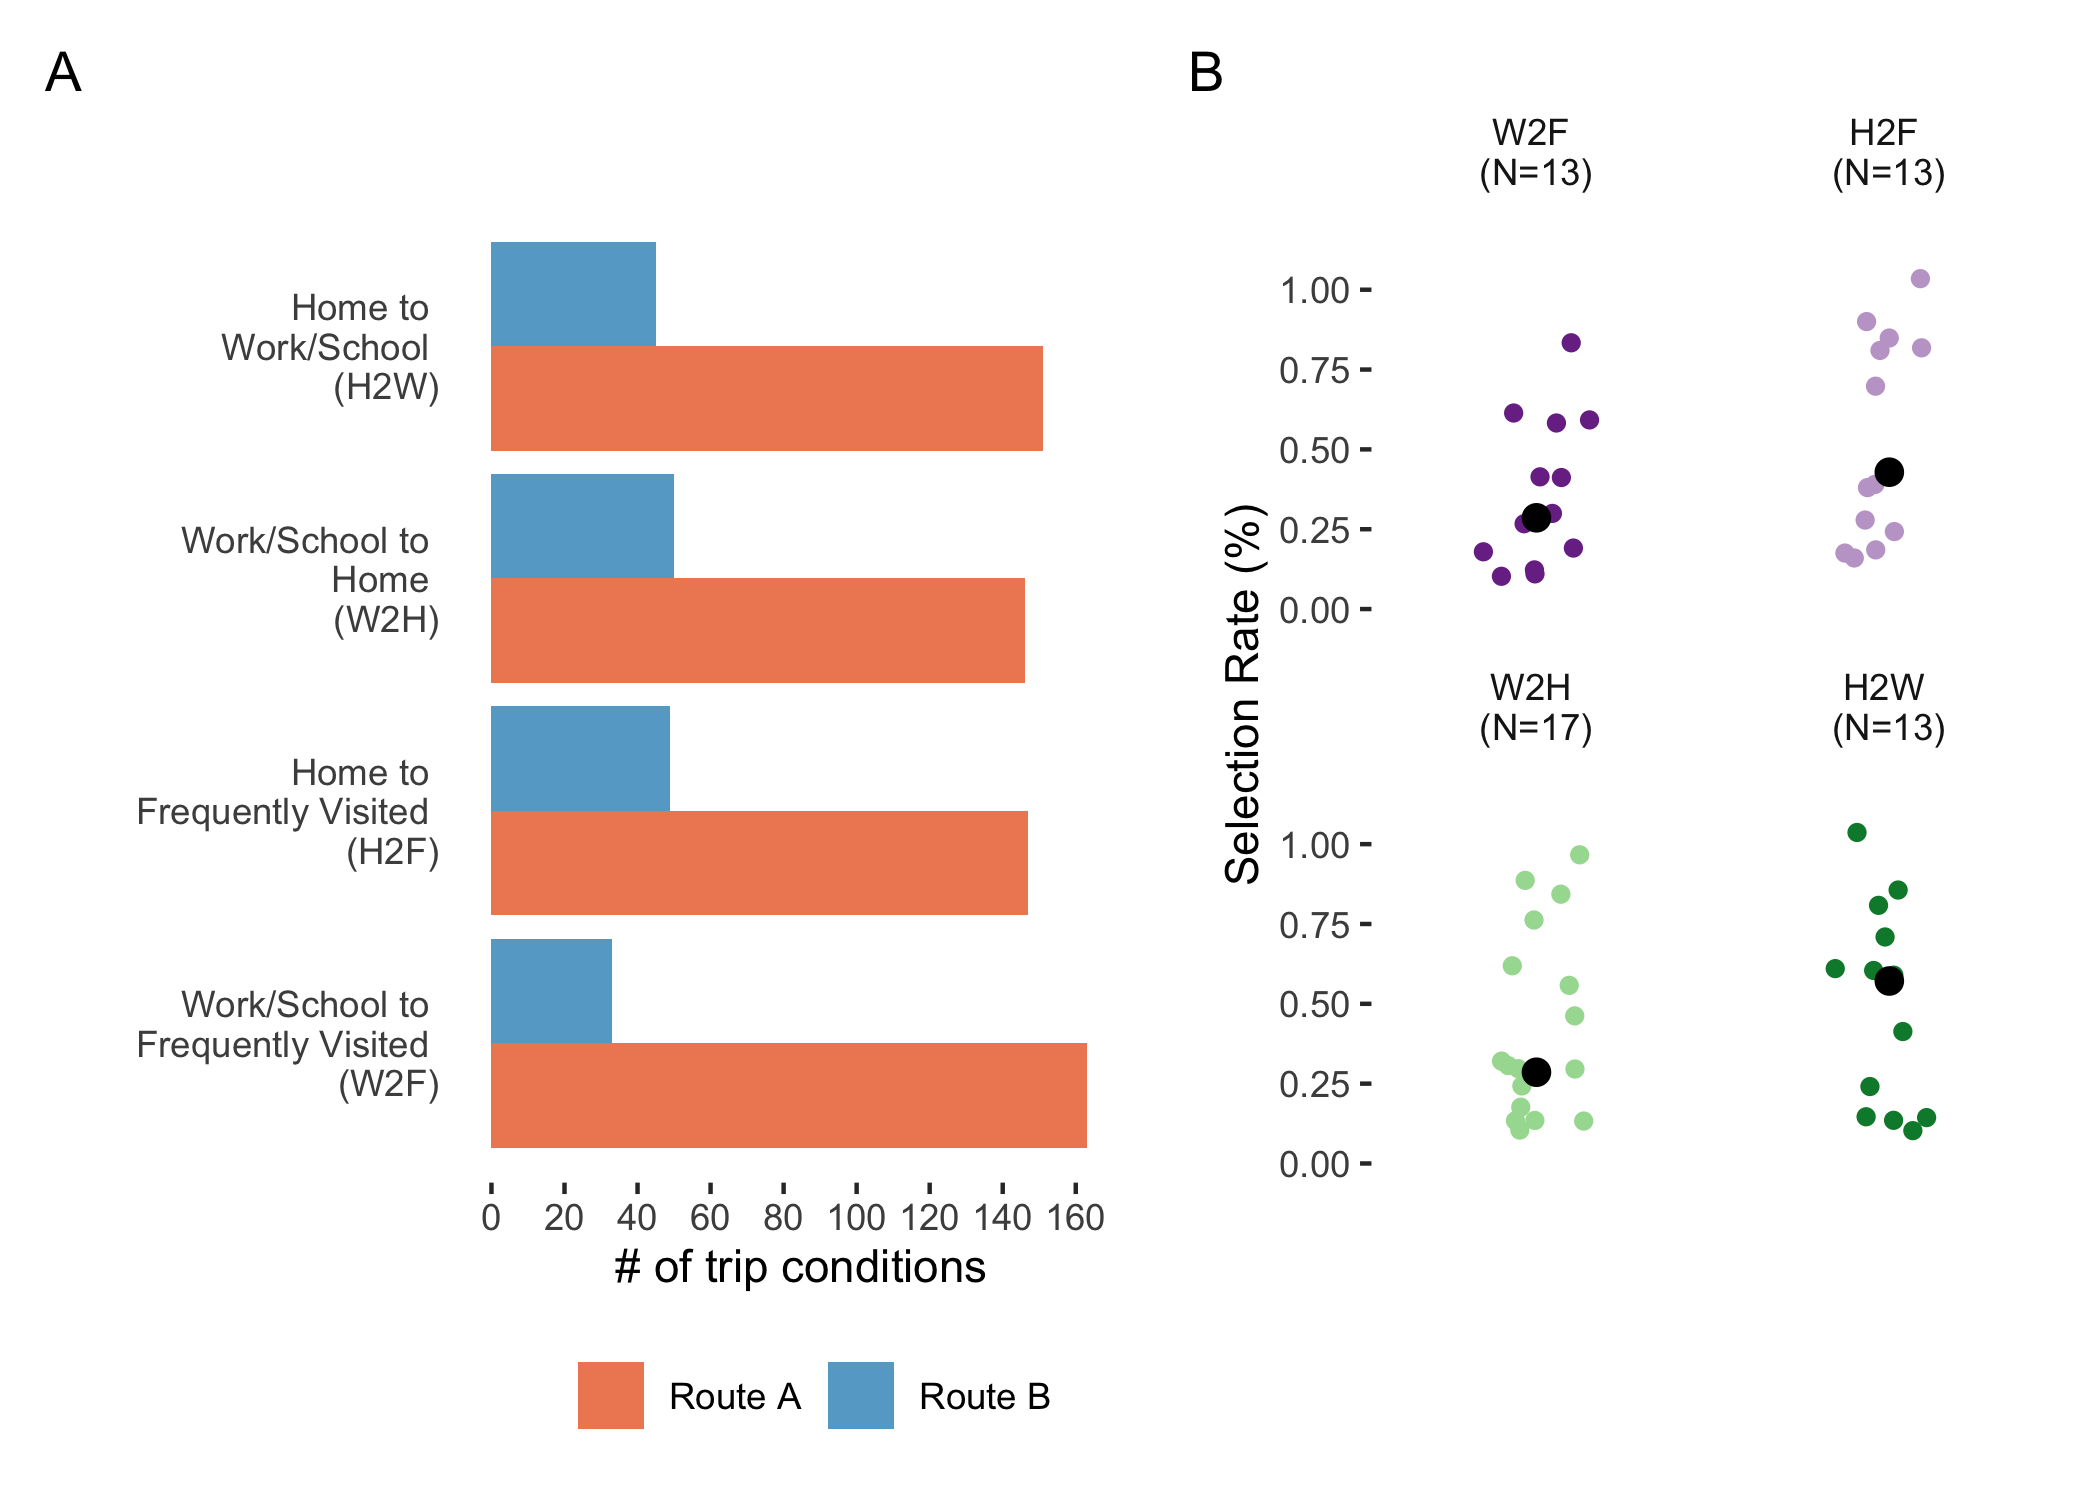
\includegraphics[scale=.2]{figures/s3-rc-unselfishratebytriptype.png}
  \caption{A) The number of trip conditions in which the participant chose each route and distributed by the trip scenario/type. B) The rate by which participants selected Route B under a trip scenario/type. The black dot shows the median selection rate.}~\label{fig:s3-rc-unselfishratebytriptype}
\end{figure}

When they are under different trip scenarios or types (Figure \ref{fig:s3-rc-unselfishratebytriptype}A), participants selected the unselfish route more when they plan to go from work or school back to their homes (N=50) and when they leave home to go to a frequently visited location (N=49) like shopping malls or groceries. Route B was selected the least when they are going from work or school to a frequently visited place (N=33). For each of the four (4) trip scenario or type, a participant selected a route for seven (7) times, with a different design version each time. Looking at their selection rates, there were more participants that chose the unselfish route at least once when they drive from work or school to their homes (N=17). But overall, trips from home going to work or school had the highest median selection rate of 57.1\% ($\mu$ =  0.495) among participants. This suggests that regardless of the design version, they were more consistent in choosing the unselfish route in this trip scenario. 

\begin{figure}[h]
\centering
  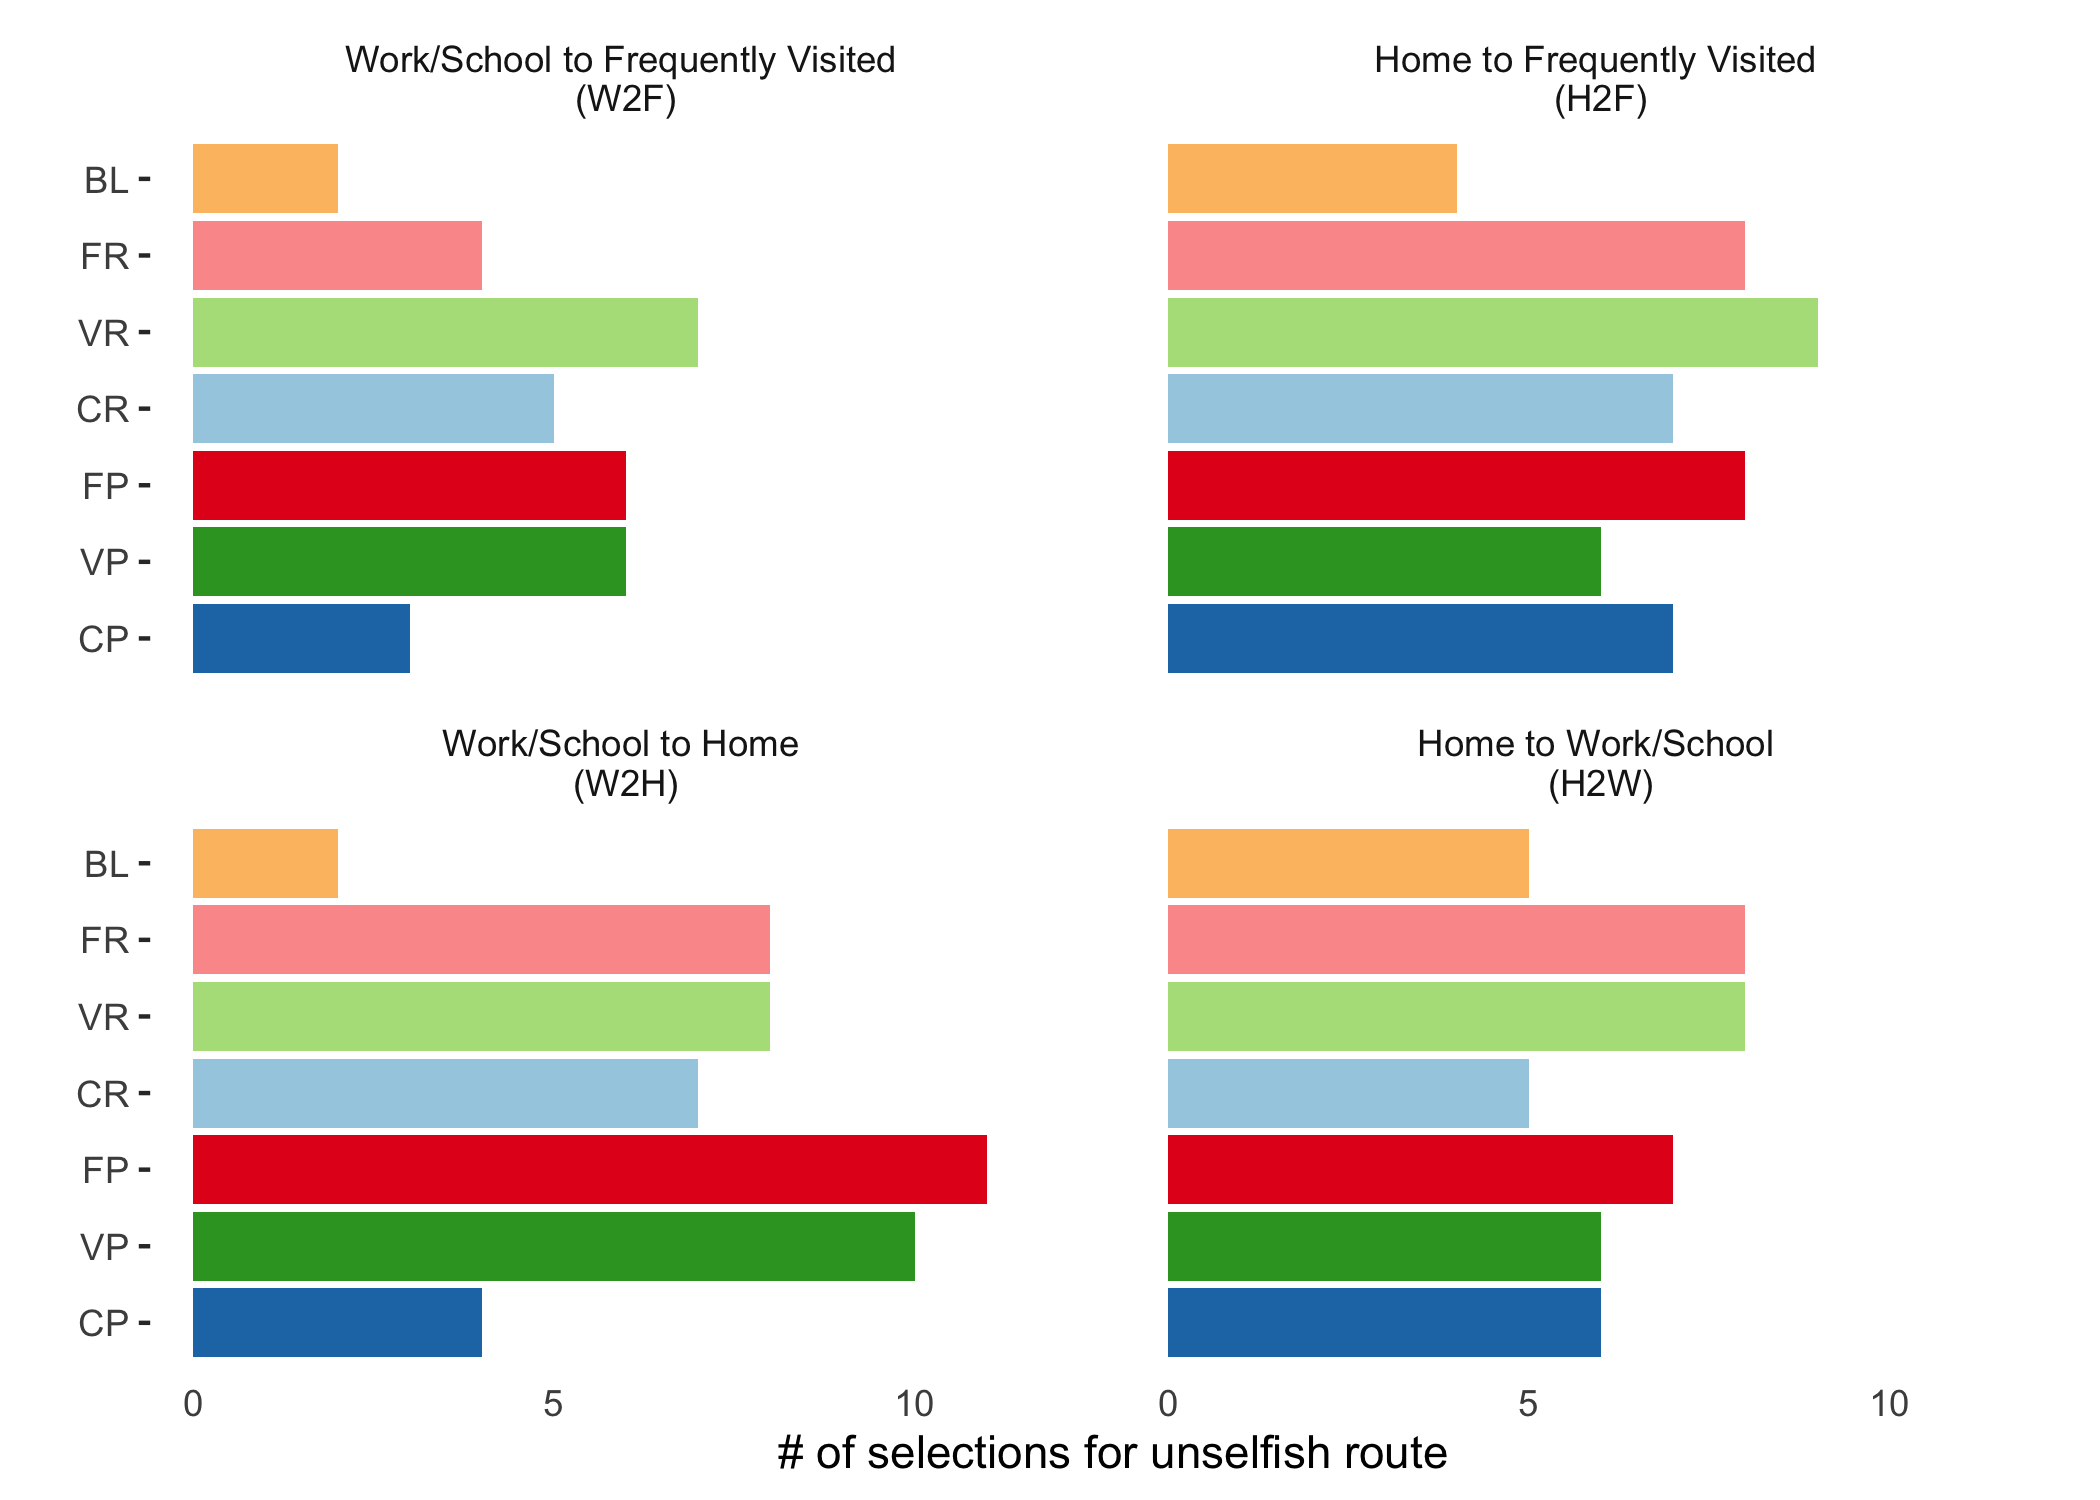
\includegraphics[scale=.2]{figures/s3-rc-unselfishinteract.png}
  \caption{The number of times the unselfish route (Route B) was chosen under each trip scenario and design version.}~\label{fig:s3-rc-unselfishinteract}
\end{figure}

But how do each design version perform under different trip scenarios? In Figure \ref{fig:s3-rc-unselfishinteract}, we can see the number of times the unselfish route was chosen when shown a specific design version. This was further distributed among the different trip scenarios. In terms of success rate, 11 or 39\% of the participants selected the unselfish route when the \textbf{FP} design version was shown in the work to home (W2H) trip scenario. Across the different trip scenarios, there was consistently more than 25\% of participants that select the unselfish route when they were shown the \textbf{VR} design version. It also has the highest success rate among the design versions in the W2F (25\%), H2F (32\%) and H2W (29\%) trip scenarios. This suggests and echoes the general utility of the valence or positive gain information in encouraging drivers to select the unselfish route. 

\subsubsection{Modeling Route Choice}
As mentioned, a Generalized Estimating Equation (GEE) model was fitted to help us compute for the likelihood of drivers in choosing the unselfish route under different trip scenarios and design versions. Because our route choice task produced binary discrete choice data, the binary logit link was used. Here, the outcome variable is the decision to follow the unselfish route or not. I want to model the main effects and two-way interactions of three predictor variables, namely trip scenario, motivative information, and familiarity information. After fitting with different correlation structures, the exchangeable correlation structure was used because it had the best model fit with a QIC\cite{pan2001akaike} value of 779. The coefficients with siginificant effects are shown in Table \ref{tab:s3-gee-significant}. 

\begin{table}[t]
    \caption{Results of the GEE model with significant main and interaction effects. The full table with all terms are in Table \ref{tab:s3-gee} in Appendix \ref{AppendixA}.}
	\label{tab:s3-gee-significant}
	\centering
	\begin{tabular}{llllll}
        \hline\hline
        Variable Name & Estimate & SE & Wald & Pr(\textgreater{}|W|) & \\
        \hline
        \textbf{(Intercept)} & \textbf{-1.7918} & \textbf{0.5401} & \textbf{11.01} & \textbf{0.00091} & \textbf{***} \\
        & & & & & \\
        \textbf{Valence} & \textbf{1.2040} & \textbf{0.5519} & \textbf{4.76} & \textbf{0.02916} & \textbf{*}  \\
        \textbf{Framing} & \textbf{1.3564} & \textbf{0.4788} & \textbf{8.02} & \textbf{0.00461} & \textbf{**} \\ 
        & & & & & \\
        \textbf{H2W * Framing} & \textbf{-1.1558} & \textbf{0.4741} & \textbf{5.94} & \textbf{0.01477} & \textbf{*}  \\
        \textbf{H2F * Framing} & \textbf{-1.1741} & \textbf{0.5807} & \textbf{4.09} & \textbf{0.04317} & \textbf{*}  \\
        & & & & & \\
        \textbf{Framing * Road Names} & \textbf{-1.1741} & \textbf{0.5501} & \textbf{4.56}  & \textbf{0.03280} & \textbf{*}   \\
        & & & & & \\
        \textbf{H2W * Framing * Road Names} & \textbf{1.5832} & \textbf{0.6418} & \textbf{6.08}  & \textbf{0.01363} & \textbf{*}   \\
        \hline
    \end{tabular}
\end{table}

Among the three factors, only the motivative information had a significant main effect, specifically when the valence is shown ($\beta$=1.2040, p<0.01) and  simple positive framing ($\beta$=1.3564, p<0.001) is used. Among the interaction terms between trip type and motivative information, there are significant interaction effects when drivers are travelling from their homes (H2W and H2F) and they are shown a simple positive framing of the unselfish route. There is also a significant interaction effect when simple positive framing is used with the list of familiar road names ($\beta$=-1.741, p<0.01). Lastly, there is a significant 3-way interaction effect when drivers travel from their home to work or school and the unselfish route is presented with both simple positive framing and list of familiar road names ($\beta$=1.5832, p<0.01). 

In terms of likelihood (Table \ref{tab:s3-gee-or}), the odds ratio shows that drivers are around 3.3 times more likely to choose the unselfish route if valence information is shown. When simple positive framing (i.e. ``\textit{Faster for everyone}'') is shown, the chances are 3.9 times more likely for the unselfish route. However, when simple positive framing is used when drivers are driving from their homes to their work, school or frequently visited location, the likelihood of following an unselfish route drops by around 0.31 to 0.31 times. It is also becomes less likely when simple positive framing is shown with the list of familiar road names (about 0.31 times less likely) in most trip types. But if that combination is used in a trip from their homes to their work or school, drivers are 4.9 times more likely to choose the unselfish route again. 

\subsection{Design Version Preference}
From the results of the pairwise comparison task, a Loglinear Bradley-Terry model was created to analyze the design version preferences using the R package \verb|prefmod|\cite{hatzinger2012prefmod}. The model is fitted using a generalized non-linear model (GNM) and estimates the likelihood or worth estimate of each design version. The sum of the worth estimates are always equal to 1. 

\begin{figure}[h]
\centering
  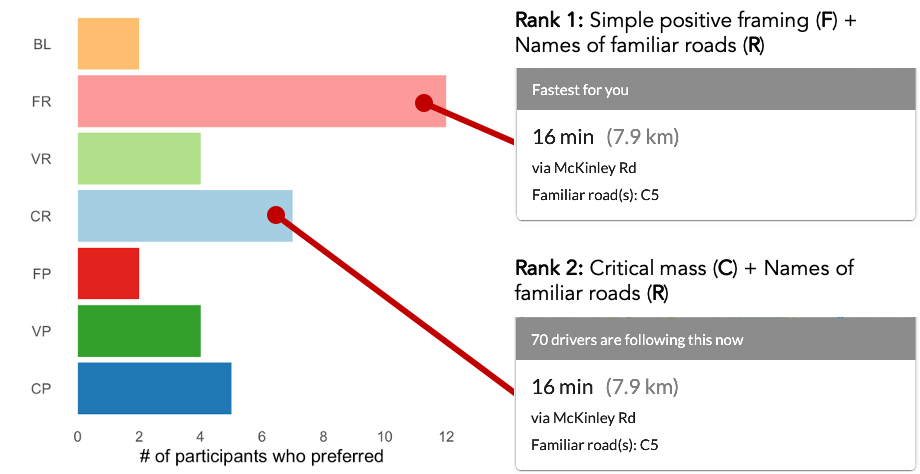
\includegraphics[scale=.8]{figures/s3-pc-winners.png}
  \caption{The absolute number of participants who preferred each design version. Note that there were ties with at most 2 versions.}~\label{fig:s3-pc-winners}
\end{figure}

Looking at the most preferred design version of each participant, there was no consensus on the best design version (Figure \ref{fig:s3-pc-winners}). In a plurality, the \textbf{FR} design version that uses simple positive framing and lists the names of familiar roads was the most preferred (N = 11). This was followed by the \textbf{CR} design version which shows the number of drivers following the route and also lists the names of familiar roads (N = 7). Among the three motivative information, design versions that use simple positive framing (\textbf{F}) was most preferred (N = 13). Between the two types of familiarity information, the versions that lists the names of familiar roads (\textbf{R}) was most preferred (N = 22). From these absolute numbers, it is indicative that drivers would be more encouraged to follow a recommended unselfish route if the presented additional information is simpler to process and explicit like the names of familiar roads. 

Remarkably, all versions were chosen by at least one participant and there were participants who still preferred the baseline version (N = 2). There were also ties between 2 design versions. These were usually between versions that use either the same motivative  (e.g. FP and FR) or familiarity (e.g. CR and VR) information. 

\subsubsection{Overall Worth Estimates}

\begin{figure}[h]
\centering
  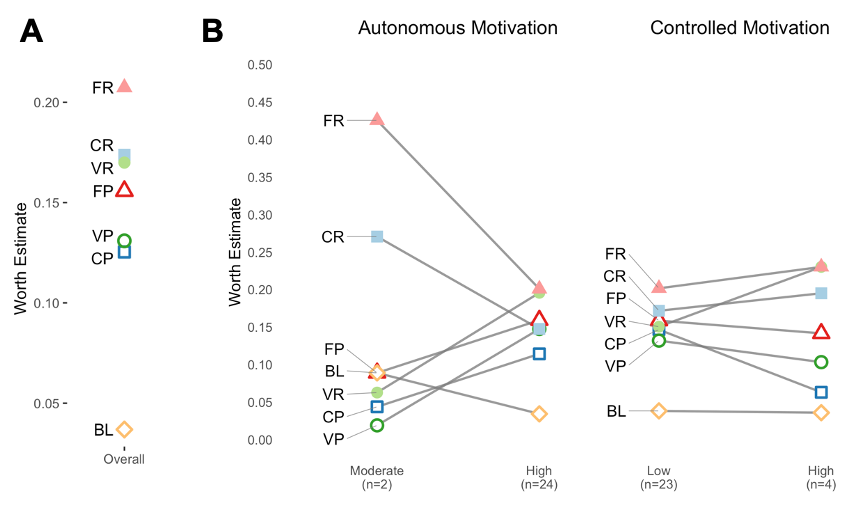
\includegraphics[scale=.9]{figures/s3-worth-overall-motivation.png}
  \caption{The worth estimates of each design version. A) On the left is the plot of preferences without considering other factors. B) On the right is the plot of preferences of participants based on their autonomous and controlled motivation scores. Only score categories with more than 1 participant were included in the plot.}~\label{fig:s3-worth-overall-motivation}
\end{figure}

Looking at the fitted model, all design versions were more preferred than the baseline version with significant differences in worth estimates (Figure \ref{fig:s3-worth-overall-motivation}A). Because the model uses the ranking of all versions from each participant, the estimated preferences have some differences from the absolute numbers discussed before. Here, the \textbf{FR} (p>0) and \textbf{CR} (p>0) design versions have the highest worth estimates which is consistent with its ranking in Figure \ref{fig:s3-pc-winners}. The marked differences are with the worth estimates of the \textbf{VR} (p>0), \textbf{FP} (p>0) and \textbf{CP} (p>0) versions. This suggests that even though \textbf{CP} was most preferred by more people, those who did not prefer it ranked \textbf{CP} lower compared to \textbf{VR} and \textbf{FP}. 

In Figure \ref{fig:s3-worth-overall-motivation}A, it is also shown that versions that lists the names of familiar roads (\textbf{FR}, \textbf{CR}, \textbf{VR}) were significantly more preferred than the baseline compared to those that just show the number of familiar roads. It might be because there is greater recall when they see the road names, which helps in their decision making. And among the motivative information types, simple positive framing (\textbf{F}) is always preferred, followed by the critical mass (C) and valence (V) information.

\subsubsection{Worth Estimates by Behavioral Regulation Type}
I was also interested to see if there are differences in worth estimates based on their behavioral regulation type. I fitted another model which had the autonomous and controlled motivation scores as subject covariates. Because the model only accepts categorical data for subject covariates, these two scores were binned into low, moderate and high categories. Those below 3 are considered low scores, while those above 3 are coded as high scores. Scores that are exactly 3 are considered moderate. 

Figure \ref{fig:s3-worth-overall-motivation}B shows the worth estimates for participants with moderate to high autonomous motivation, and low and high controlled motivation scores. The \textbf{FR} design version was consistently preferred the most but in this case, the differences are not significant. Only the preferences of people with high autonomous motivation for \textbf{CP} (p<0.05), \textbf{VP} (p<0.001) and \textbf{VR} (p<0.05) design versions were shown to be significant. 

\subsubsection{Worth Estimates by General Causality Orientation}
\begin{figure}[h]
\centering
  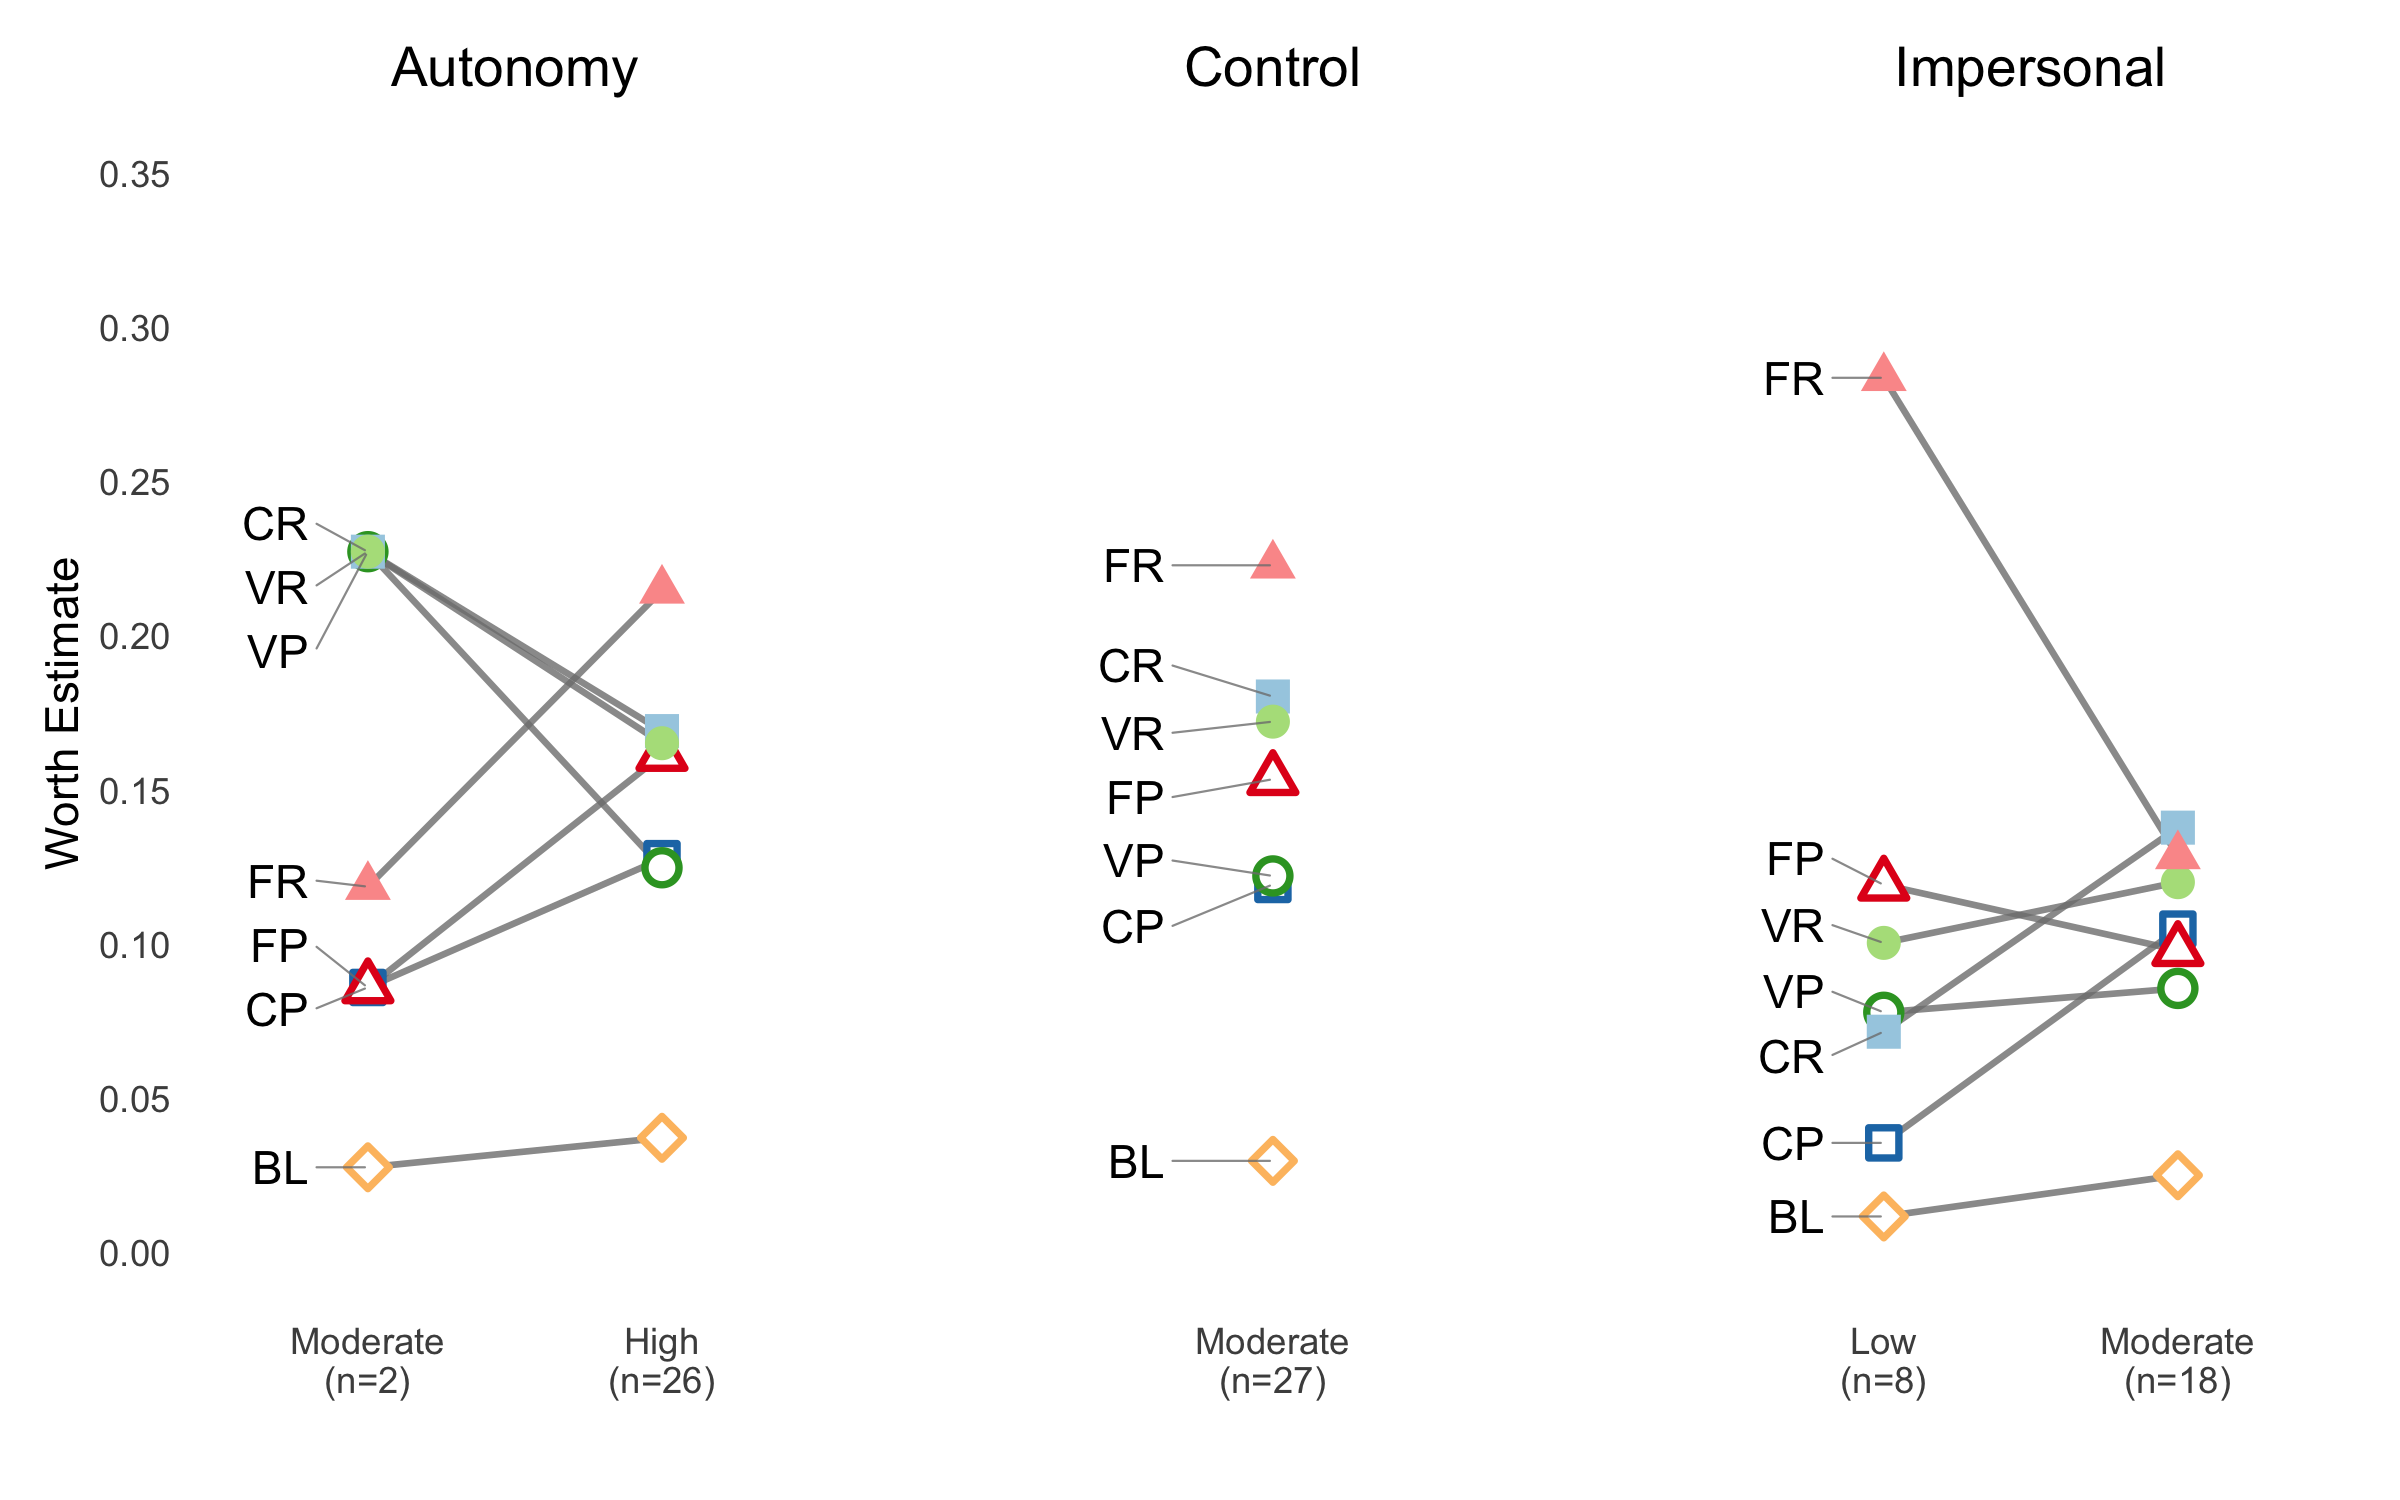
\includegraphics[scale=.18]{figures/s3-worth-gcos.png}
  \caption{The worth estimates of each design version when the general causality orientation is considered. Only score categories with more than 1 participant were included in the plot.}~\label{fig:s3-worth-gcos}
\end{figure}

Considering people's general causality orientation, Figure \ref{fig:s3-worth-gcos} shows that the \textbf{FR} design version would most likely encourage participants with high autonomy orientation, moderate control orientation and low impersonal orientation to take the recommended unselfish route. However, only those with moderate control orientation have shown significant preference.

Looking at the autonomy orientation, there were significant preferences for the \textbf{CR} (p<0.05), \textbf{VR} (p<0.05) and \textbf{VP} (p<0.05) design versions for those with moderate scores. The rest are non-significant. 

The worth estimates for participants with moderate control orientation all have significant differences (p<0) compared to the baseline. Remarkably, the order of preference closely resembles that of the overall model.

In terms of impersonal orientation, participants with low scores showed significant preference for the \textbf{FR} design version (p<0.05). For those with moderate scores, the \textbf{CR} design version (p<0) was the most preferred, followed by the \textbf{FR} version. This and all other worth estimates showed significant differences compared to the baseline (p<0). 

\subsection{Comparison of Stated Route Choice and Preference}
Knowing their most preferred design versions from the pairwise comparison task, did the participants really choose the unselfish route when those were presented to them in the route choice experiment? Out of the 21 participants who selected the unselfish route at least once, only eighteen (18) of them were consistent with their most preferred design version. They had an average selection rate of 26\% when presented with their most preferred design version. Two participants selected the unselfish route in all four (4) times that their most preferred was used. On the other hand, three (3) participants never selected it.

\section{Towards Better Adoption of Unselfish Routes}
This study provides insights into how Self-Determination Theory can be used to identify and design motivative information that can help increase the likelihood that drivers will select an unselfish route. Here I present the key findings from the results from the results. 

\subsection{Case for Autonomy Support}
In this study, the main design goal was to ensure that the different design versions are autonomy-supportive. In Self-Determination Theory, that means the environment or tool has to address the three basis psychological needs, namely autonomy, competence and relatedness. That is how I decided to incorporate the three motivative information used in the prototypes: a simple positive framing of choosing unselfishly, the critical mass of active drivers currently following the recommended routes, and the positive gain in everyone's travel time if at least one driver chooses an unselfish route. With a participant pool that mostly have high autonomy orientation and high autonomous motivation scores, it should be expected that almost all of them would choose the unselfish route at least once. However, the stated route choice results only show partial support. Although 75\% of participants selected the unselfish route at least once, it should be noted that all seven (7) participants who chose the optimal route completely have high autonomy orientation and high autonomous motivation scores. So it would be interesting to unpack this counter-intuitive behavior in future studies. 

Despite that, the majority who choose unselfishly at least once included participants who have moderate autonomy orientation and low to moderate autonomous motivation. Results suggest that the design versions were able to facilitate the internalization of extrinsic motivation and positively influence the choice of unselfish routes, which supports the case for autonomy support in driving navigation applications.

\subsection{Simplicity and Explicitness}
Considering both stated route choices and preferences, the design version that combines simple positive framing and the list of familiar roads showed universal positive utility in increasing the likelihood of choosing an unselfish route. In terms of preference, the \textbf{FR} design version was the most preferred except for participants that reported moderate autonomy orientation. Design versions with either simple positive framing or the list of familiar roads also resulted to higher selection rates for the unselfish route regardless of trip scenario/type. This design version can convince more drivers compared to other versions but it might not be as successful in motivating them to continue with their unselfish choices. These can all be attributed to the simplicity of the messaging that immediately conveys the positive benefit of making the unselfish choice. The explicitness of listing the names of some familiar roads also helped in the positive response to this design version. Showing the familiar road names can help drivers reduce the need to recall and make them easily recognize what is familiar to them. 

The valence information also helped motivate participants to choose unselfish routes. Although not many participants chose unselfishly when they were shown design versions that use this motivative information, they showed the most consistency regardless of the trip type. Also from the GEE model, it is shown that participants were 3 times more likely to choose the unselfish route when shown information about the positive gain of everyone. However, the current message that reads ``Avg Travel Time of everyone can be \verb|N| min faster'' might have different interpretations from drivers. In the interviews, some participants recall that they were not sure whether the displayed estimated travel time for them would also be reduced by some minutes. Although it is now suggested to convey uncertainty when showing predicted values, especially for transparency, this messaging had some effect as to whether they would consider this information for decision making or not.

\subsection{Need for Relatedness}
Looking at the version preferences, the \textbf{CR} design version consistently ranks second to the \textbf{FR} version. This suggests that even though the participant pool are mostly with high autonomy orientation and high autonomous motivation, they still highly prefer a design version that addresses their need for relatedness. In SDT, this is the psychological need of a person to feel connected and interdependent with others. The critical mass information was chosen specifically for that purpose. Commonly used in e-commerce websites, this motivative information make people feel they are about to belong to a group of other individuals when they perform a task. The participants with moderate impersonal and control orientation mostly prefer the use of the \textbf{CR} design version. This might be because they have a weak tendency to leave things as it is. It might encourage them more to choose unselfishly if they explicitly see how much impact they can have in the system, which is by joining a smaller number of drivers taking the unselfish route. The same need can also be said for participants with moderate autonomy orientation. However, the current messaging for the unselfish route that reads ``30 drivers are following this now'' might have different interpretations for drivers. For one participant, they avoided the unselfish route because they thought more drivers would choose this since there are less people. 

\subsection{Personalized Motivation}
Although the \textbf{FR} design version was the most preferred, the results from the stated route choice experiment reveals that a personalized motivation and messaging might be required to ensure that drivers will consistently or at least be more inclined to choose the unselfish route. This was also supported by the fact that there was no clear winner in ensuring consistent and high selection rate across trip types, causality orientation and behavioral regulatory styles. 

In particular, a personality-targeted design\cite{nov2013personality,moon2002personalization} might be worth exploring but with a focus on using SDT constructs since we are dealing with motivation. One inspiration could be the work of Grau et. al.\cite{grau2018personalized} in which they used personalized motivation-supportive messages to help increase the number of reported community issues. One challenge for this approach is the collection of proper data to inform the personalization. It could be achieved either through proxy variables within the context of driving or navigation, or the simplification of the GCOS and MVS surveys so that users do not have to answer long forms at the beginning of their driving navigation experience. 

\section{Limitations and Future Work}
This study focused on collecting stated route choices using online surveys. Although ecological validity was maintained by using the real home, work and frequently visited locations of recruited participants, the trip scenarios were still hypothetical contexts. Aside from that, the recommended routes gathered from Google Maps that were used in the prototypes were taken at days and times that might not match when the participant would actually answer the survey forms. The 28 conditions were given to participants in 7 working days. Because it follows a within-subject study design, this approach was intended to avoid respondent fatigue and learning effect. However, there were still participants who forgot to answer on a daily basis and had to answer more than one (1) survey form in a day. While it is totally out of our control, this might have affected some of their answers. Lastly, the pairwise comparison was done by the same participants in the stated route choice experiment. Ideally, more respondents should answer it to have a more statistically significant result.

I also envision several directions for future work, specifically on the messaging and presentation of the proposed motivative and familiarity information, and the use of other types of information that drivers might consider in trip planning and navigation. In my design versions, the motivative and familiarity information were purely text displayed below the map. While that works to control confounding effects from other factors (i.e. color, form) and let the participants focus on the value of the information, it leaves little creativity for more different ways of presenting the proposed motivative and familiarity information on the navigation application. The current prototype design also makes the area below the map too cluttered with text. As the primary goal of this study is to increase the likelihood of choosing an unselfish route, additional work needs to be done in exploring whether some of these information can be presented on the map, along with the display of the route. We also have to acknowledge the fact that most drivers do visual inspection using the interactive map more than checking the texts of navigational information presented below it.

Another critical avenue for exploration is improving the messaging if the proposed motivative and familiarity information are found to be better presented as text to users. In the current prototype, the wording are based on certain assumptions about language use and culture of the recruited participants. However, results from the interviews have shown that the current messaging had different interpretations among participants which had an effect on their stated route choices. Future exploration might want to consider co-design with drivers and serious consultation with communications experts in order to achieve proper messaging. 

Finally, future explorations might also consider using more practical navigational and contextual information. My proposed motivative information are prosocial in nature, intended to highlight the potential choice's benefit to other people and society as a whole. It might be worth considering the addition of contextual information such as the number of traffic lights and or the estimated waiting times. This could provide a balance of information that could highlight a potential unselfish choice's benefit to drivers and others while still being familiar to them.

\section{Conclusion}
In this chapter, I focus on the trip planning step of the navigation task and explored adding motivative information to encourage drivers to choose an unselfish route. Guided by the Self-Determination Theory, I used three types of motivative information: the simple positive framing of a potential choice's benefit to the driver and others, the critical mass or the number of drivers who chose the recommended routes, and the positive valence or the decrease in everyone's travel time. Using insights from Chapter \ref{ChapterInteractNavi} on what drivers mostly value in choosing a route to follow, I also explored adding two types of familiarity information: the absolute number of familiar roads, and the names of a few familiar roads. In a stated route choice experiment, I investigated the effects of trip types, motivative information and familiarity information on the likelihood that the unselfish route will be chosen before a trip begins. After this, a pairwise comparison task was also conducted. This is to estimate which combination of motivative and familiarity information is the most preferred in encouraging drivers to choose an unselfish route. My results show that drivers are more likely to choose an unselfish route when the motivative and familiarity information are simple and explicit, like the combined use of simple positive framing and names of familiar roads. Although there is universal positive utility for this combination, my results also suggests that a personality-targeted motivation and messaging would be ideal especially if we want to cater to different trip scenarios and to people with different causality orientations and behavioral regulatory types. 